%chktex-file 46 
%%turn off the syntax check on $...$
\documentclass[a4paper,fleqn]{cas-sc}% fleqn stands for "flush left equations"
%%%%%%%%%%%%%%% Declare Package: %%%%%%%%%%%%%
\usepackage[authoryear,longnamesfirst]{natbib}
\usepackage[export]{adjustbox}
\usepackage{ragged2e}% Align macro package
\usepackage{amsmath,amssymb}
%%% Nomenclature packages %%%%%%%%%
\usepackage{framed,multicol}% frame and multi-column package in the double column for nomenclature
\usepackage{nomencl}% use nomenclature package
\makenomenclature
\setlength{\nomitemsep}{-\parskip} % Baseline skip between items
\renewcommand*\nompreamble{\begin{multicols}{2}}
\renewcommand*\nompostamble{\end{multicols}}
%%%%%%%%%%%%%%%%%%%%%%%%%%%%%%%%%%%%%%%%%%%%%%%%%%
\graphicspath{{Figures/}}% the path of graphs1
% \usepackage{bm}% bold font special for math formulas
\usepackage[name=Fig,labelsep=period]{caption}
% \usepackage[raggedright,nooneline,FIGTOPCAP]{subfigure}% need to call both packages: subcaption and caption at the same time
\usepackage{setspace}
\DeclareMathOperator\dif{d\!}% the derivative operator d
\usepackage{xfrac}% small fraction, for example 1/2
\usepackage{multirow,booktabs} %three-line table
\usepackage{array} % fixed width and auto newline(wrap) as well centering
\usepackage{callouts}%% annotation for figures
\usepackage{microtype}% improve the intervals between words to make typing more beautiful
\usepackage{lineno,hyperref}% display line number, use hyper reference
\usepackage{nameref}

%%%%%%%%%%%%%% Title and author: %%%%%%%%%%%%%
\begin{document}
\let\WriteBookmarks\relax
\def\floatpagepagefraction{1}
\def\textpagefraction{.001}
\shorttitle{Unequal planet load sharing}
\shortauthors{Feng et~al.}
\title[mode = title]{A vibration signal model of planetary gearboxes with unequal load sharing among planets}
\author[1]{Haoqun Ma}[type=editor]
\address[1]{University of Science and Technology Beijing, No.30, Xueyuan Road, Haidian District, Beijing.}
\author[1]{Zhipeng Feng}[orcid=0000-0002-3403-4386]
\cormark[1]
\cortext[cor1]{Corresponding author}%
\ead{fengzp@ustb.edu.cn}%
% 
%%%%%%%%%%%%%% Abstract %%%%%%%%%%%%%%%%%%%%%%
\begin{abstract}
    Planetary gearboxes feature large transmission ratios within compact volumes because they can divide the input torque load into parallel paths formed by planets. Unevenly load sharing among planets leads to inefficiency and accelerating fatigue. This paper establishes a vibration signal model to describe how the uneven distribution of planet loads affects the vibration signal composition. The derived Fourier spectrum illustrates the contacting planet number affects the system natural vibration and spectral structure. we also discuss the influences of different planet numbers, input torques, and manufacturing error severity. Numerical simulation and experimental substations agree well with the proposed theoretical model.
\end{abstract}
%%%%%%%%%%%%%%%%% Highlights %%%%%%%%%%%%%%%%%%%%%%
\begin{highlights}
    \item Vibration signal model of equal load sharing among planets
    \item Influence of gear meshing vibration, transfer path effects and natural frequency
    \item Analytical expression of Fourier spectrum 
    \item Explanation on spectral configuration arisen from different factors
\end{highlights}
%%%%%%%%%%%%%%%% keywords %%%%%%%%%%%%%%%%%%
\begin{keywords}
    Unequal load sharing \sep\ Planetary gearbox \sep\ Signal model \sep\ Fault diagnosis
\end{keywords}
    
%%%%%%%%%%%%%% Begin document: %%%%%%%%%%%%%%%
\maketitle
%%%%%%%%%%%%%%% Custom commands: %%%%%%%%%%%%
\setcitestyle{square}
\def\degree{${}^{\circ}$}
\def\myscale{0.5}
%%%%%%%%%%%%%%% Introduction %%%%%%%%%%%%%%%%
\section{Introduction}
\par Planetary gearboxes have several planets forming parallel transmission paths to split the input torque. This configuration reduces the load applied to the at each meshing gear and allow the planetary gearboxes to be compact. Because of the co-axial structure of planetary gearboxes, radial forces acting on the gears can be neutralized. And flexibly supported sun gears and carrier can move radially at a certain degree to compensate for the manufacturing errors partially. These above mentioned merits of planetary gearboxes will compromise if the loads are unevenly applied to planets, usually arisen from manufacturing errors, such as a planet pinhole deviating from its nominal position. Unequal load sharing can also lead to inefficiency or accelerating wear. 
\par  Most of works  on the fault diagnosis of planetary gearboxes mainly concern gears \cite{Feng2012} or bearings \cite{Zhao2019}, and do no involve the planet load sharing, though the planet load sharing also significantly impacts the vibration signals.
\par Many investigations focus on the calculation of load sharing factors and the physical mechanism. Some conclusions contributed by previous publication are summarized as follows \cite{Singh2010511-530}:
\begin{itemize}
    \item The floating (piloting) sun gear can improve the conditions of planet equal load sharing \cite{seager1970}.
    \item Load sharing characteristics are primarily affected by the tangential errors, and insensitive to radial errors \cite{Bodas2004}. 
    \item Three planet gearboxes with at least one floating central members can evenly distribute the load if the manufacturing errors are within a certain range \cite{Singh2010511-530}.
    \item The diagonal planets in four-planet gearboxes have the same load sharing \cite{Ligata2008}.
    \item Planet load sharing essentially a quasi-static problem and does not need to consider dynamic effects \cite{Kahraman1994}.
    \item Increasing the input torque can alleviate the planet load inequality \cite{Ligata2008}.
    \item Increasing the planet number without tightening manufacturing error tolerance will deteriorate the load sharing condition \cite{Singh2005}.
\end{itemize}
\par Vibration signal modelling can bridge between the physical mechanism of the system and the mathematical expression both in time domain and frequency domain, facilitating the further fault diagnosis of unequal load sharing and other components. McFadden and Smith \cite{McFadden1985} probably firstly proposed that the asymmetry sidebands around the meshing frequency is ascribed to the planet revolution motion relative to the fixed transducer mounted on the ring gear. The established models of vibration signal indicates the planet number multiples of carrier order in spectrum are arisen from the planet motion. This feature originates from the signal acquisition method but not the inherent vibration of planetary gearboxes. Inalpolat and Kahraman \cite{Inalpolat2009} took planet phases into account and classified planetary gearboxes into five classes according to their planet angular positions (equally spaced or unequally spaced) and phases conditions (in phase, sequentially spaced, arbitrary phases). Mark and Hines \cite{Mark2009} derived the Fourier-series spectrum of fixed transducer response mounted on the ring gear and well explained the unequal load sharing will lead to the harmonics at non planet number multiples of tooth meshing. Lei \cite{Lei2016} et al. proposed a phenomenological model containing the meshing vibration between the sun gear and planets as well as the effects of gear faults, further verifying the conclusions in Mark's paper.
\par The vibration signal model proposed in this paper based on and extends these models in the above references. We  can find that natural vibration excited by the gear meshing cannot be omitted, because it globally shapes the signal envelope in frequency domain. In addition, the assumption that all planets are engaging with sun or ring gear is invalid in cases where the manufacturing errors are severe or the input torques are relatively low, especially for planet number is more than four. When some planets lose connection with sun or ring gears, the natural frequency will also shifts due to the decreased system stiffness. The derived Fourier spectrum with these considerations can better agree with the practical circumstances. As the planet number, error severity and input torque vary, the signal model and its corresponding spectral evolves. All these factors will be discussed in this paper.
\par Section \ref{sec:signal_model} introduces the vibration signal model. The Fourier spectrum is derived in Section \ref{sec:spectral_structure}. Section \ref{sec:factor_discussion} discusses the influence of main factors in the signal model. Experimental verification is presented in Section \ref{sec:experimental_validation}. At last, Section \ref{sec:conclusions} concludes the above investigation. 
%%%%%%%%%%%%%%% References %%%%%%%%%%%%%%%%%
%%%%%%%%%%%%%%% Principle %%%%%%%%%%%%%%%%
\section{Signal model \label{sec:signal_model}}

    
    %%%%%%%%%%%%%%%%% nomenclature Display %%%%%%%%%%%%
\begin{table*}[!t] 
    \begin{framed} 
        \printnomenclature
    \end{framed}
\end{table*}
\nomenclature{\(f_{\rm m}\)}{gear meshing frequency}
\nomenclature{\(f_{\rm c}\)}{carrier rotation frequency}
\nomenclature{\(J\)}{inertia moment}
\nomenclature{\(k(t)\)}{stiffness}
\nomenclature{\(L_i\)}{load sharing ratio of the \(i\)-th planet}
\nomenclature{\(k_e\)}{effective support stiffness concerning both the bearing and gear meshing}
\nomenclature{\(r_s\)}{sun gear pitch radius}
\nomenclature{\(T_s\)}{total torque applied on input sun gear}
    \begin{figure*}
        \centering
        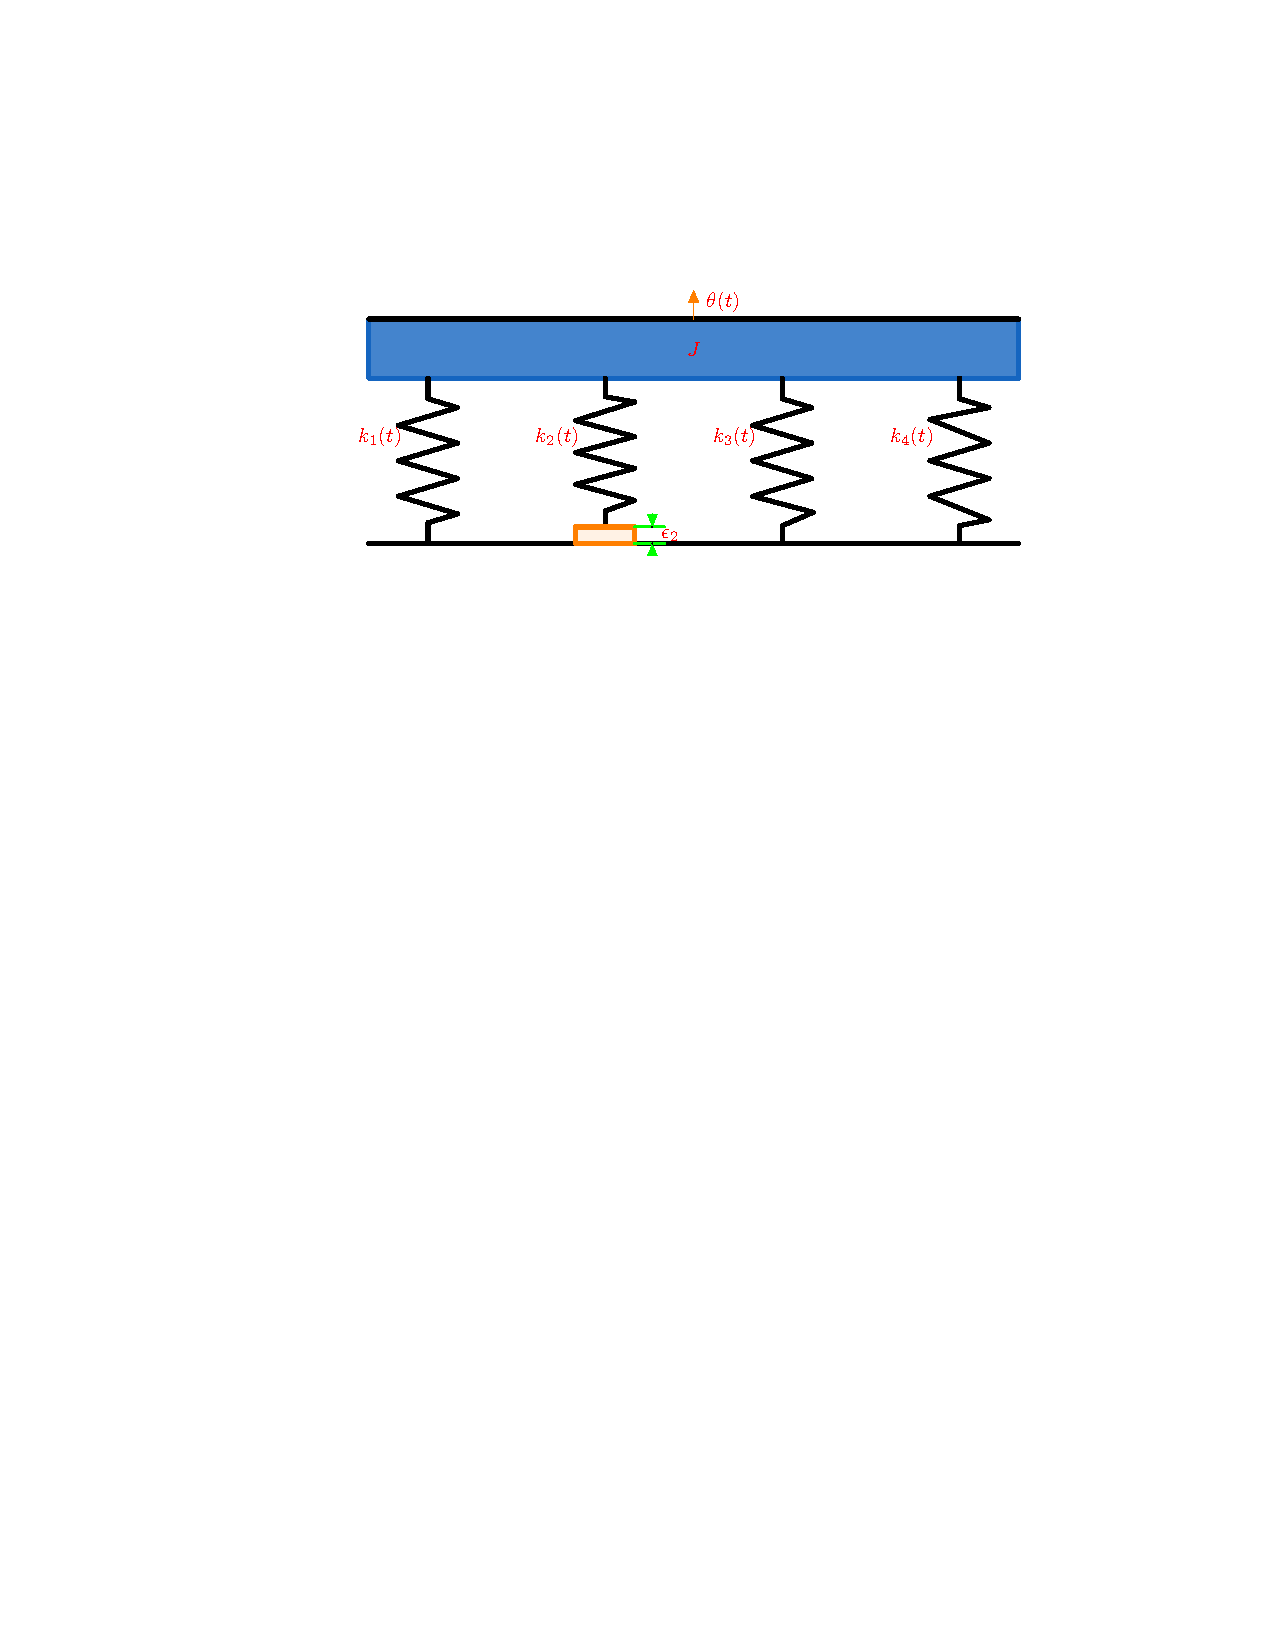
\includegraphics[scale=0.6,width=0.8\textwidth,height=1.6in]{spring_mass.pdf}
        \caption{Vibration system of unequal load sharing among four planets.}
    \label{fig:vibration_system_of_spring_mass}
    \end{figure*}
\subsection{General signal model}
\par A typical layout of planetary gearboxes consists of three kinds of gears mounted so that the centers of planet gears revolves around the center of sun and ring gears. This paper merely discusses the common cases of speed reducers where the sun gear connects with the power input shaft and the carrier works as power output, while vibration sensors are usually mounted on the surface of the stationary ring gear in diagnostic applications. 
% \begin{figure}[pos=htbp]
%     \centering
%     \begin{annotate}{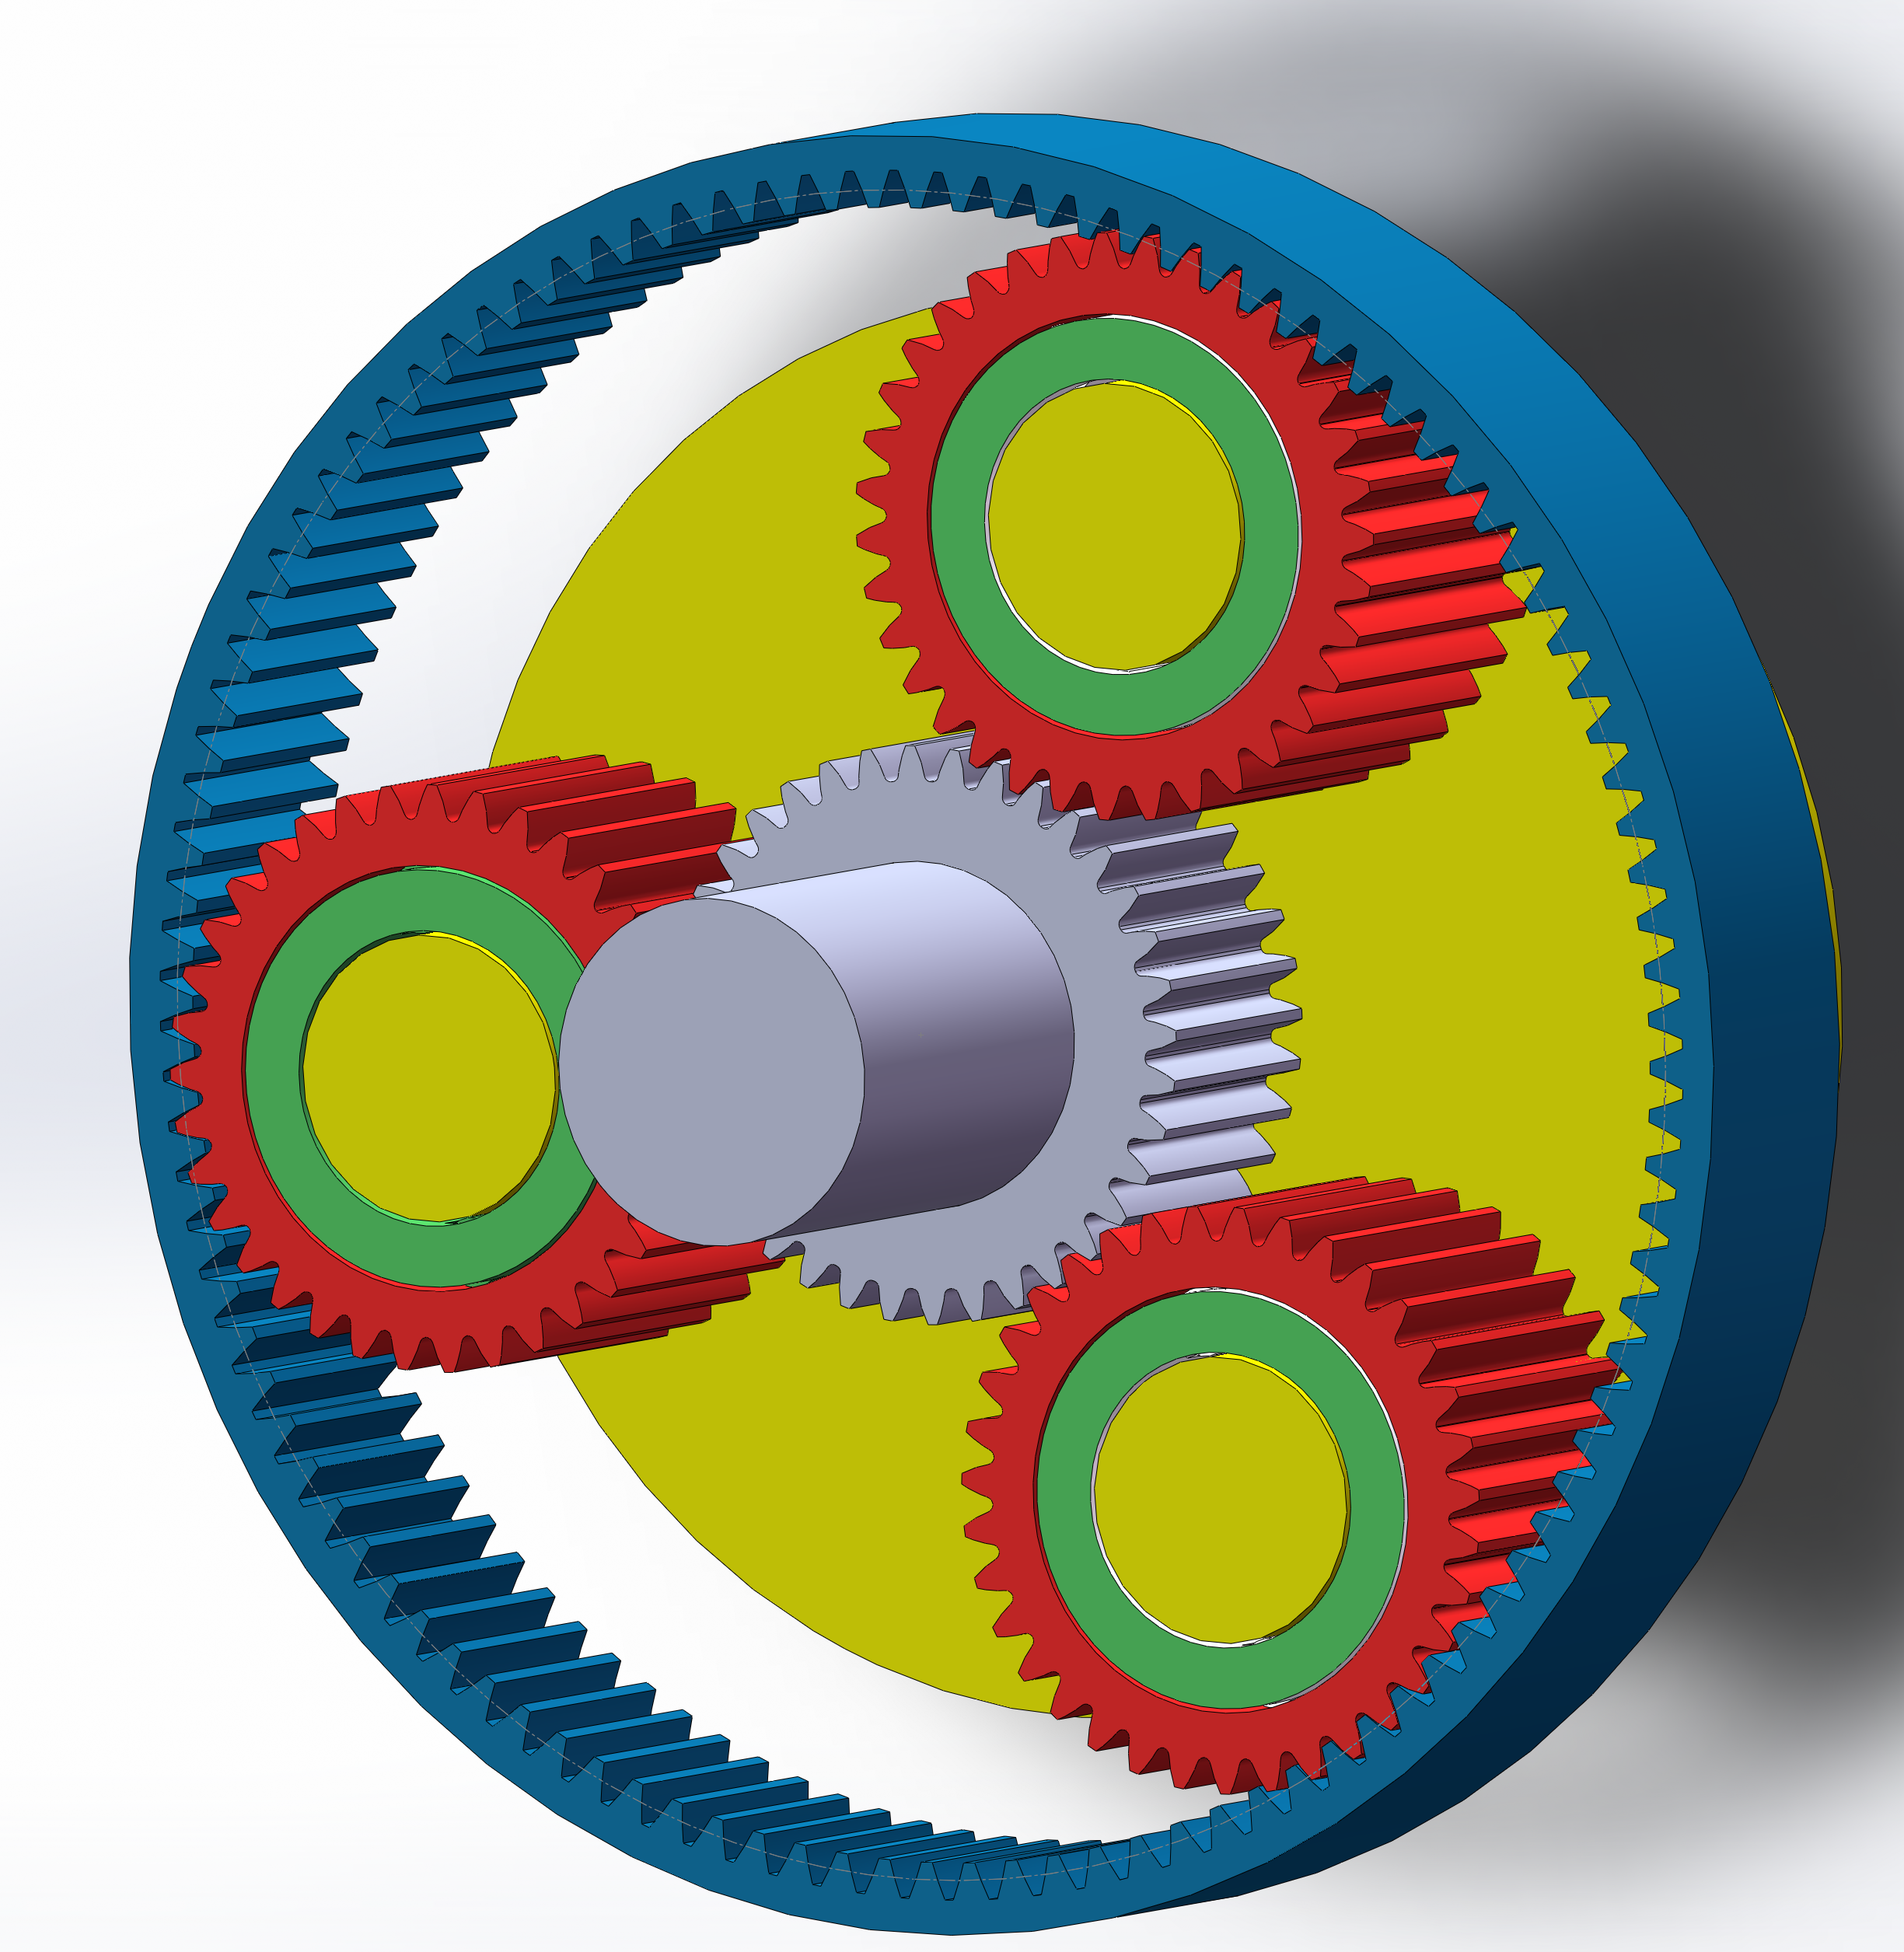
\includegraphics[width=0.3\textwidth]{Planetary_Gearbox.PNG}}{0.3}
%         \callout{-8,-7}{Ring gear}{-5,-5.8}
%         \callout{8,-7}{Planet gear}{4,-5.5}
%         \callout{-8,7}{Sun gear}{-0.8,1.2}
%         \callout{8,7}{Carrier}{4.5,1}
%     \end{annotate}
%     \caption{Configuration of planetary gearboxes.}
%     \label{fig:planetary_gearbox_layout}
% \end{figure}
\par The vibration in planetary gearboxes mainly origins from the meshing of gears \cite{Velex1996}. When the planet gears engage with the ring gear or sun gear, the number of the involved tooth varies with the relative rotation between gears and their contact stiffness changes consequently. The transmission load nominally remains constant and the gearbox is a parametrically excited multi-degree-freedom system \cite{Acar2019}. 
\par The signal model perceived by the stationary transducer on the gearbox housing can be modelled as the summation of all planet vibration considering transfer path effects. The impulsive intensity of gear meshing is assumed to proportional to the load applied on each planet. The vibration of each planet is divided into planet-ring and planet-sun parts. Thus, the general signal model is
\begin{equation}
    x(t)=\sum_{i=1}^{M} L_i \cdot \left[ \sigma_{{\rm r}i}(t) \xi_{{\rm r}i}(t) + \sigma_{{\rm s}i}(t) \xi_{{\rm s}i}(t) \right], \label{eq:general_signal}
\end{equation}
where $M$ is the planet number, $L_i$ denotes the load sharing coefficient, $\sigma_{\rm pr}$ and $\sigma_{\rm ps}$ denotes transfer path effect on planet-ring and planet-sun gears, respectively, $\xi_{{\rm r}i}$ and $\xi_{{\rm s}i}$ are the vibration originating from the $i$-th planet-ring and planet-sun gears.
\par Nominally, all planet center distribute along circumference of the carrier evenly. Without loss of generality, the nominal angular position of first planet center is set as zero, and
\begin{equation}
    \Theta_i=\frac{(i-1)\cdot 2\pi}{M},
\end{equation}
where $\Theta_i$ denotes the nominal position of $i$-th planet. In addition, due to the manufacturing or assembling process, each planet center deviates from the nominal position by $\epsilon_i$. If $\epsilon_i>0$, the planet engages with the ring or sun gear in advance, or negative error represents the engagement lag. We can assume $\epsilon_1=0$ in the coordinate system, because these planets locate relatively to each other. Even if $\epsilon_1 \neq 0$, we can also set $\epsilon_i=\epsilon'_i-\epsilon'_1,i \geq 2$, where $\epsilon'_i$ is $i$-th planet error in another coordinate system.
\par To reveal the spectral structure simply, the gear meshing vibration of each planet is regarded as Dirac comb function $\operatorname{III}(t)=\sum_{i=-\infty}^{+\infty}\delta(t-i)$. The meshing frequency can be calculated by different engaging gears,
\begin{equation}
    f_{\rm m}=Z_{\rm r} \cdot (f_{\rm r}+f_{\rm c})=Z_{\rm p} \cdot (f_{\rm p}-f_{\rm c})=Z_{\rm s} \cdot (f_{\rm s}-f_{\rm c}). \label{eq:meshing_frequency}
\end{equation}
where $\{\}_{\rm r}$, $\{\}_{\rm p}$, $\{\}_{\rm s}$, $\{\}_{\rm c}$ denote ring gear, planet, sun gears and carrier, respectively; $Z_{\{\}}$ is the gear number and $f_{\{\}}$ is the rotating frequency. 
\par For planet-ring gears, the planet angular position error bring about the time shift. The time shift is the angular error divided by the relatively rotating velocity. Thus, the planet-ring meshing vibration can be written as
\begin{equation}
    \xi_{{\rm r}i}(t)=A_{{\rm r}i}\operatorname{III}\left[f_{\rm m} \cdot (t-\frac{\epsilon_i+\Theta_i}{2 \pi f_{\rm c}})\right],\label{eq:planet-ring_meshing}
\end{equation}
where $A_{{\rm r}i}$ is the impulsive amplitude of $i$-th planet-ring gear meshing, the $f_{\rm m}$ is the meshing frequency. Park et al. propose the difference between planet-ring and planet-sun meshing phase \cite{Parker2004}. Similarly, the planet-sun meshing vibration is
\begin{equation}
    \xi_{{\rm s}i}(t)=A_{{\rm s}i} \operatorname{III}\left[f_{\rm m} \cdot (t + \frac{\epsilon_i+\Theta_i}{2 \pi f_{\rm s}- 2 \pi f_{\rm c}})+ \frac{\varphi_i}{2 \pi} \right],\label{eq:planet-sun_meshing}
\end{equation}
where $A_{{\rm r}i}$ is the impulsive amplitude of $i$-th planet-sun gear meshing, $\varphi_i$ is the phase difference between planet-ring and planet-sun meshing for the $i$-th planet.
%%%%%%%%%%%%%%%%%%%%%%%% Algorithm of load sharing factors %%%%%%%%%%%
\subsection{Algorithm of load sharing factors\label{sec:algorithm_load_sharing}}
\par Ligata et al. proposed an algorithm to calculate the load sharing factor through analogizing the in-plane torque balance problem to the 3-D force and torque balance problem \cite{Ligata2009}.
\begin{enumerate}
    \item Initialization of parameters. Analogize the torque balance model with the planet center circle to the force and moment balance model in the axial direction perpendicular to the planet center plane.  Analogize the planet gears to springs with the same stiffness $1/k_{\rm e}=1/(k_{\rm rp}+k_{\rm sp})+1/k_{\rm b}$, where $k_{\rm rp}=2.57\times 10^8$ and $k_{\rm sp}=1.67\times 10^8$ are the meshing stiffness of planet-ring and planet-sun, respectively, $k_{\rm b}=3.2\times 10^7$ is the planet bearing stiffness. The pinhole errors is equivalent to length of spring in the axial direction $z_i=e_i=2(R_{\rm r}-R_{\rm p})\sin(\epsilon_i/2)\cos(\epsilon_i/2)$, where $R_{\rm p}$ is the planet radius, $R_{\rm s}$ is the sun radius, $\epsilon_{i}$ is the angular position error the $i$-th planet. The locations of springs accord with planet pinhole positions the planet center plane, $x_i=-(R_{\rm p}+R_{\rm s})\sin(\Theta_i+\epsilon_i)$ , $y_i=(R_{\rm p}+R_{\rm s})\cos(\Theta_i+\epsilon_i)$. The input torque equals the axial load on a plate pushing on the springs, $W=2T_{\rm s}/R_{\rm s}$.  The rocking motions $\phi_x$ and $\phi_y$ of the plate are analogous to the floating motions of the central member in the x and y directions. The radius of the circle where planet centers locate at is $R_{\rm b}=R_{\rm s}+R_{\rm p}$.
    \item Determine the initial disposition of \textit{planet center plate}. The first contacting point $J=\mathop{\arg\max}\limits_{i}(z_i)$. Define a line  tangent to the circle on plane  $P_1$ (parallel with the x-y plane) and anther point $Q$ also on the line $y_Q=-(x_Q-x_J)x_J/y_J+y_J$. Define the plane $P_2$ by three points $J, Q, K$:
    \begin{equation}
        \begin{split}
        a x+ b y+ c z+ d=0,\\
        a= \left(y_Q-y_J\right)\left(z_K-z_J\right)-\left(y_K-y_J\right) \left(z_Q-z_J\right),\\
        b=\left(x_K-x_J\right) \left(z_Q-z_J\right)-\left(x_Q-x_J\right) \left(z_K-z_J\right),\\
        c=\left(y_K-y_J\right) \left(x_Q-x_J\right)-\left(y_Q-y_J\right) \left(x_K-y_J\right),\\
        d=x_Q \left(y_J z_K-z_J y_K\right)+x_J \left(y_K z_Q-z_K y_Q\right)+x_K \left(z_J y_Q-y_J z_Q\right).
        \end{split} 
    \end{equation}
    \item Transverse all $K\neq J$ to find the second point $K$ satisfying $K=\mathop{\arg\max}\limits_{K \neq J}\left\{\arccos\left[\frac{|c|}{\sqrt{a^2+b^2+c^2}}\right]\right\}$. Define the plane  $P_3$  by the three points $J, K, N$. Recalculate the corresponding $a, b,c$ for plane $P_3$. The third point $N=\mathop{\arg\max}\limits_{N \neq J,K}\left\{\arccos\left[\frac{|c|}{\sqrt{a^2+b^2+c^2}}\right]\right\}$.
    \item Verify whether the load  application point $C$ (origin point) is within the triangle $J,K,N$ via crossing between the vectors formed by three sides, otherwise repeat the step 4.
    \item Calculate the supporting forces of three points ($J,K,N$) by applying the force and moment balance equations.
    \begin{equation}
        \begin{split}
        \sum F_i=W,\\
        M_x=\sum F_i\cdot y_i=0,\\
        M_y=\sum F_i\cdot x_i=0, \label{eq:force_equilibrium}
        \end{split}
    \end{equation}
    \item Consider the case of more than three supporting planets. Obtain the $i$-th spring deflection $\delta_i=\frac{F_i}{k_e}$. Update the coordinates on the new plane $P_d$: $z^d_i=z_i-\delta_i$, as well as the $a,b,c,d$. Recalculate the coordinates of other points.
    \item For $H\neq J,K,N$, if the origin length protrude the plane $P_d$:$z_H>z^d_H$, chose $G_1,G_2$ from $J,K,N$ to satisfy load application point $C$ is within triangel $HG_1G_2$, the other residual point is denoted by $B$. Add the following equation to the Eq. \ref{eq:force_equilibrium}.
    \begin{equation}
        F_{G_1}A_1+F_{G_2}A_2+F_B A_3 F_H A_4=k_{\rm e}Y.
    \end{equation}
    where
    \begin{equation}
        \begin{split}
            Y=[A_1,A_2,A_3,A_4] \cdot [z_{G_1};z_{G_2};z_B;z_H],\\
            \eta=\frac{(x_{G_2}-x_{G_1})(y_B-y_{G1})-(x_B-x_{G_1})(y_{G_2}-y_{G_1})}{(x_{G_2}-x_{G_1})(y_H-y_{G_1})-(x_H-x_{G_1})(y_{G_2}-y_{G_1})},\\
            A_1=(\eta-1)y_{G_2}+y_B-\eta y_H,    A_2=(1-\eta)y_{G_1}-y_B+\eta y_H,\\
            A_3=y_{G_2}-y_{G_1},A_4=y_{G_2}-y_{G_1}.
        \end{split}
    \end{equation}
    \item Repeat the step 7 for all springs in contact with the plate after the load $W$ is applied. Generally if the contacting planets are more than 3, $N_C>3$, add $N_C-3$ equations:
    \begin{equation}
        F_{G_{1m}}A_{1m}+F_{G_{2m}}A_{2m}+F_{Bm}A_{3m}-F_{Hm}A_{4m}=K_{\rm e}Y_m,\quad m\in[1,N_C-3].
    \end{equation}
    \item Finally, the load sharing factors are $L_i=F_i/W$.
\end{enumerate}
\begin{figure}[pos=htbp]
    \centering
    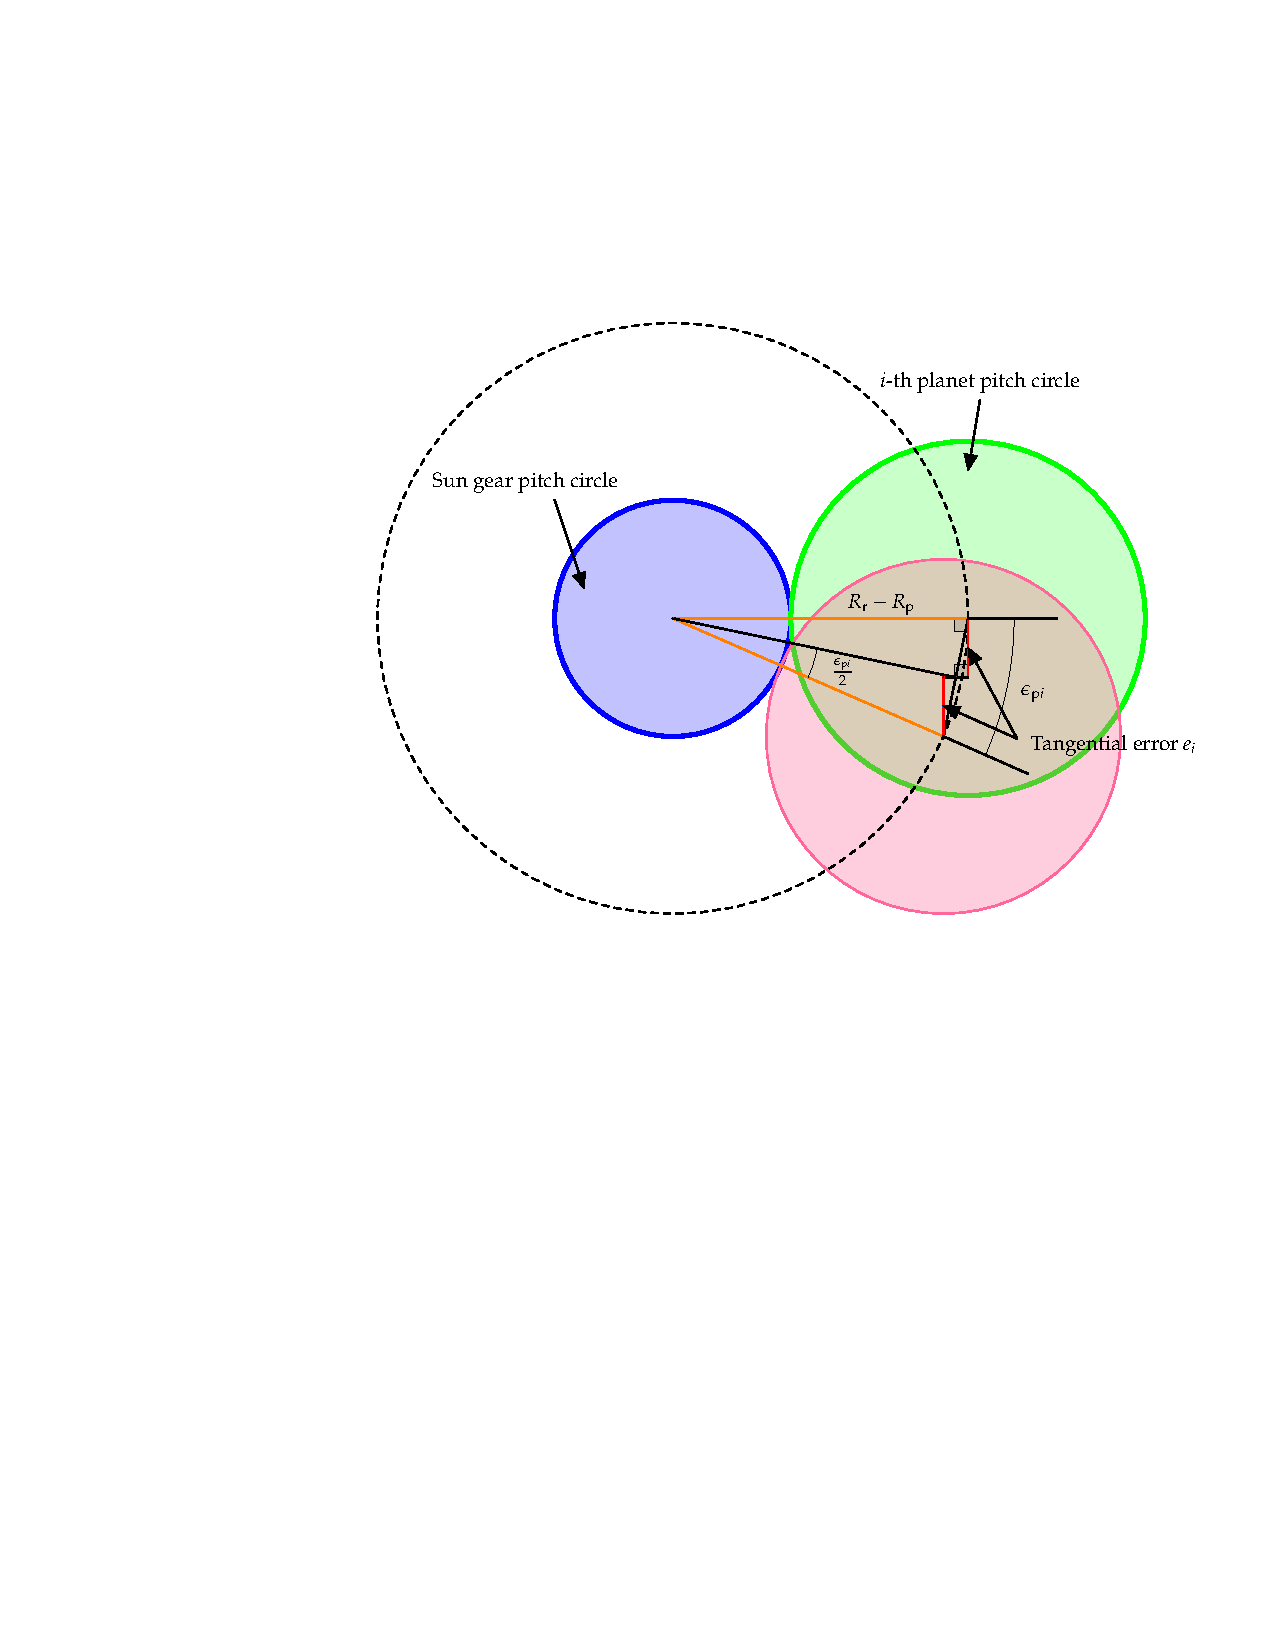
\includegraphics[scale=0.5]{tangential_error.pdf}
    \caption{Tangential error calculation (correct the $\epsilon_{pi}$)}
    \label{fig:tangential_error}
\end{figure}
\par Unequal load sharing will gives rise to non-uniform impulsive intensity. The acceleration are linearly affected by the dynamic force exerted. Thus, the vibration amplitude of each planet is assumed to be proportional to the load applied on it \cite{Inalpolat2009}. In other words, planet load modifies the amplitude of the vibration signal. Moreover, the unevenly planet distribution along the angular position of carrier also has phase modulation when the transfer path is considered simultaneously. These effects will be illustrated explicitly in the later Section \ref{sec:factor_discussion}. 
\subsection{Transfer paths\label{sec:transfer_path}}
\par The vibration originating from the planet meshing with ring or sun gear propagate through several paths to the stationary sensor mounted on the case. As demonstrated in Fig. \ref{fig:transfer_path}, there are three paths for planet-ring and planet-sun gear meshing, respectively. These transfer paths can be categorized into two types, depending on whether or not they pass through bearings. The paths passing through bearings (path 2, 3, 5, 6 in Fig. \ref{fig:transfer_path}) must transfer via the gearbox housing to reach the sensor fixed on the top. Compared with the paths merely passing through gears (path 1, 4 in Fig. \ref{fig:transfer_path}), these paths passing bearings are longer and more likely to be attenuated by the lubricating oil layer in bearings \cite{Feng2012}. To simplify modelling, only the shorter paths (path 1, 4 in Fig. \ref{fig:transfer_path}) are concerned in this paper.
\begin{figure}[pos=htbp]
    \centering
    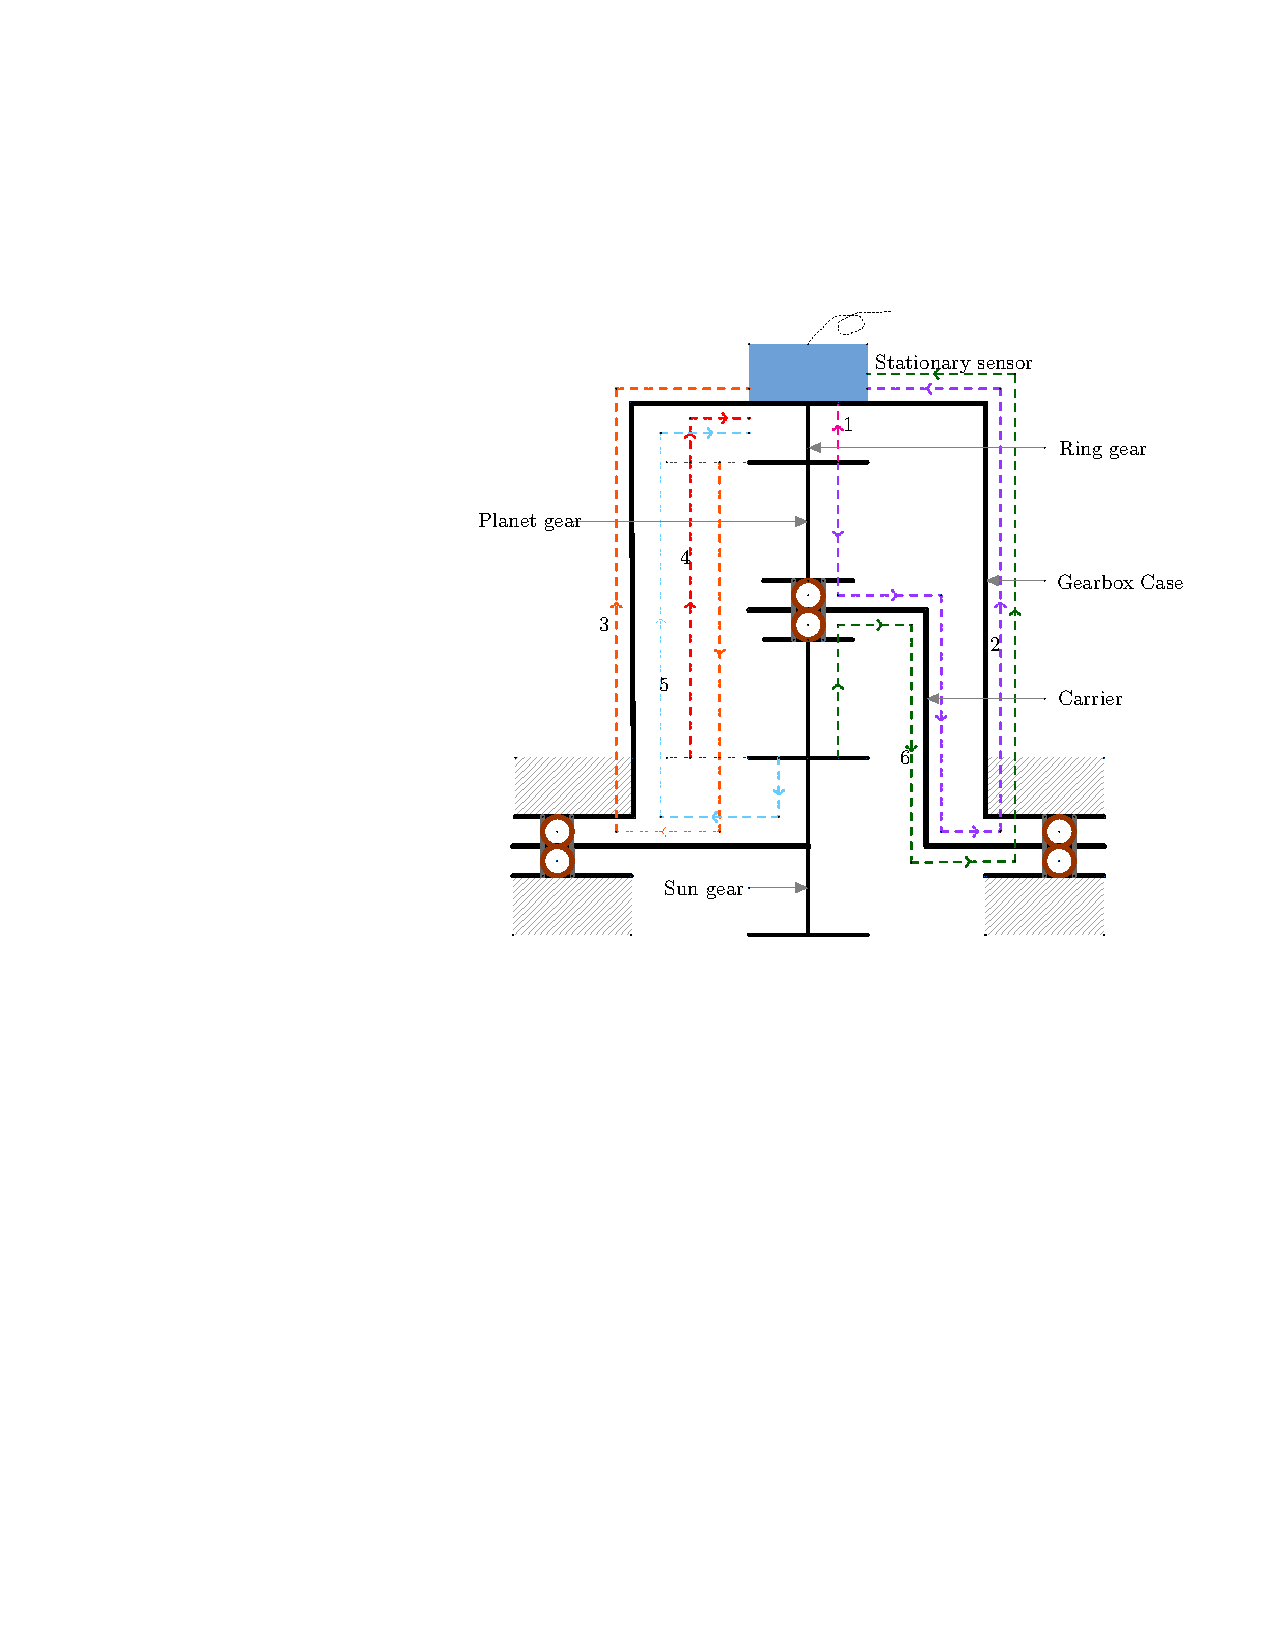
\includegraphics[scale=0.5]{transfer_path.pdf}
    \caption{Transfer paths of gear meshing vibration.\textbf{add explanation on path number. from where to where.}\label{fig:transfer_path}}
\end{figure}
\par The lengths of path 1 and path 4 vary with the circumferential position of carrier. For each planet, the meshing vibration points get close to the fixed sensor as the planet approaches the top surface of gearbox case. When the planet reach the climax of its revolution circle, the fixed transducer percepts the maximum impulsive strength. While the planet arrives at the case bottom, the perceived impulses are most weakened. The path 1 length is triangle wave of time (as shown in Fig. \ref{fig:path_length_trangle_wave}) when planetary gearboxes operate at a constant speed and planet distributes evenly, 
\begin{equation}
    l_{{\rm r}i}(t)=
    \begin{cases}
        2 \pi R_{\rm r} f_{\rm c} \left|t-(\frac{\epsilon_i+\Theta_i}{2 \pi f_{\rm c}} + \frac{n}{f_{\rm c}}) \right|, \frac{n}{f_{\rm c}} - \frac{1}{2 M f_{\rm c}} + \frac{\epsilon_i+\Theta_i}{2\pi  f_{\rm c}} \leq t < \frac{n}{f_{\rm c}} + \frac{1}{2 M f_{\rm c}} + \frac{\epsilon_i+\Theta_i}{2\pi f_{\rm c}}, n\in \mathbb{Z} , i=1,2,\ldots,M\\
        +\infty, \quad \text{otherwise}
    \end{cases},
\end{equation}
where $M$ is the planet number. The path 4 is the sum of the diameter of the planet pitch circle and $l_{{\rm r}i}$,
\begin{equation}
    l_{{\rm s}i}(t)=l_{{\rm r}i}+2 R_{\rm p}. \label{eq:path_4_length}
\end{equation}
\begin{figure}[pos=htbp]
    \centering
    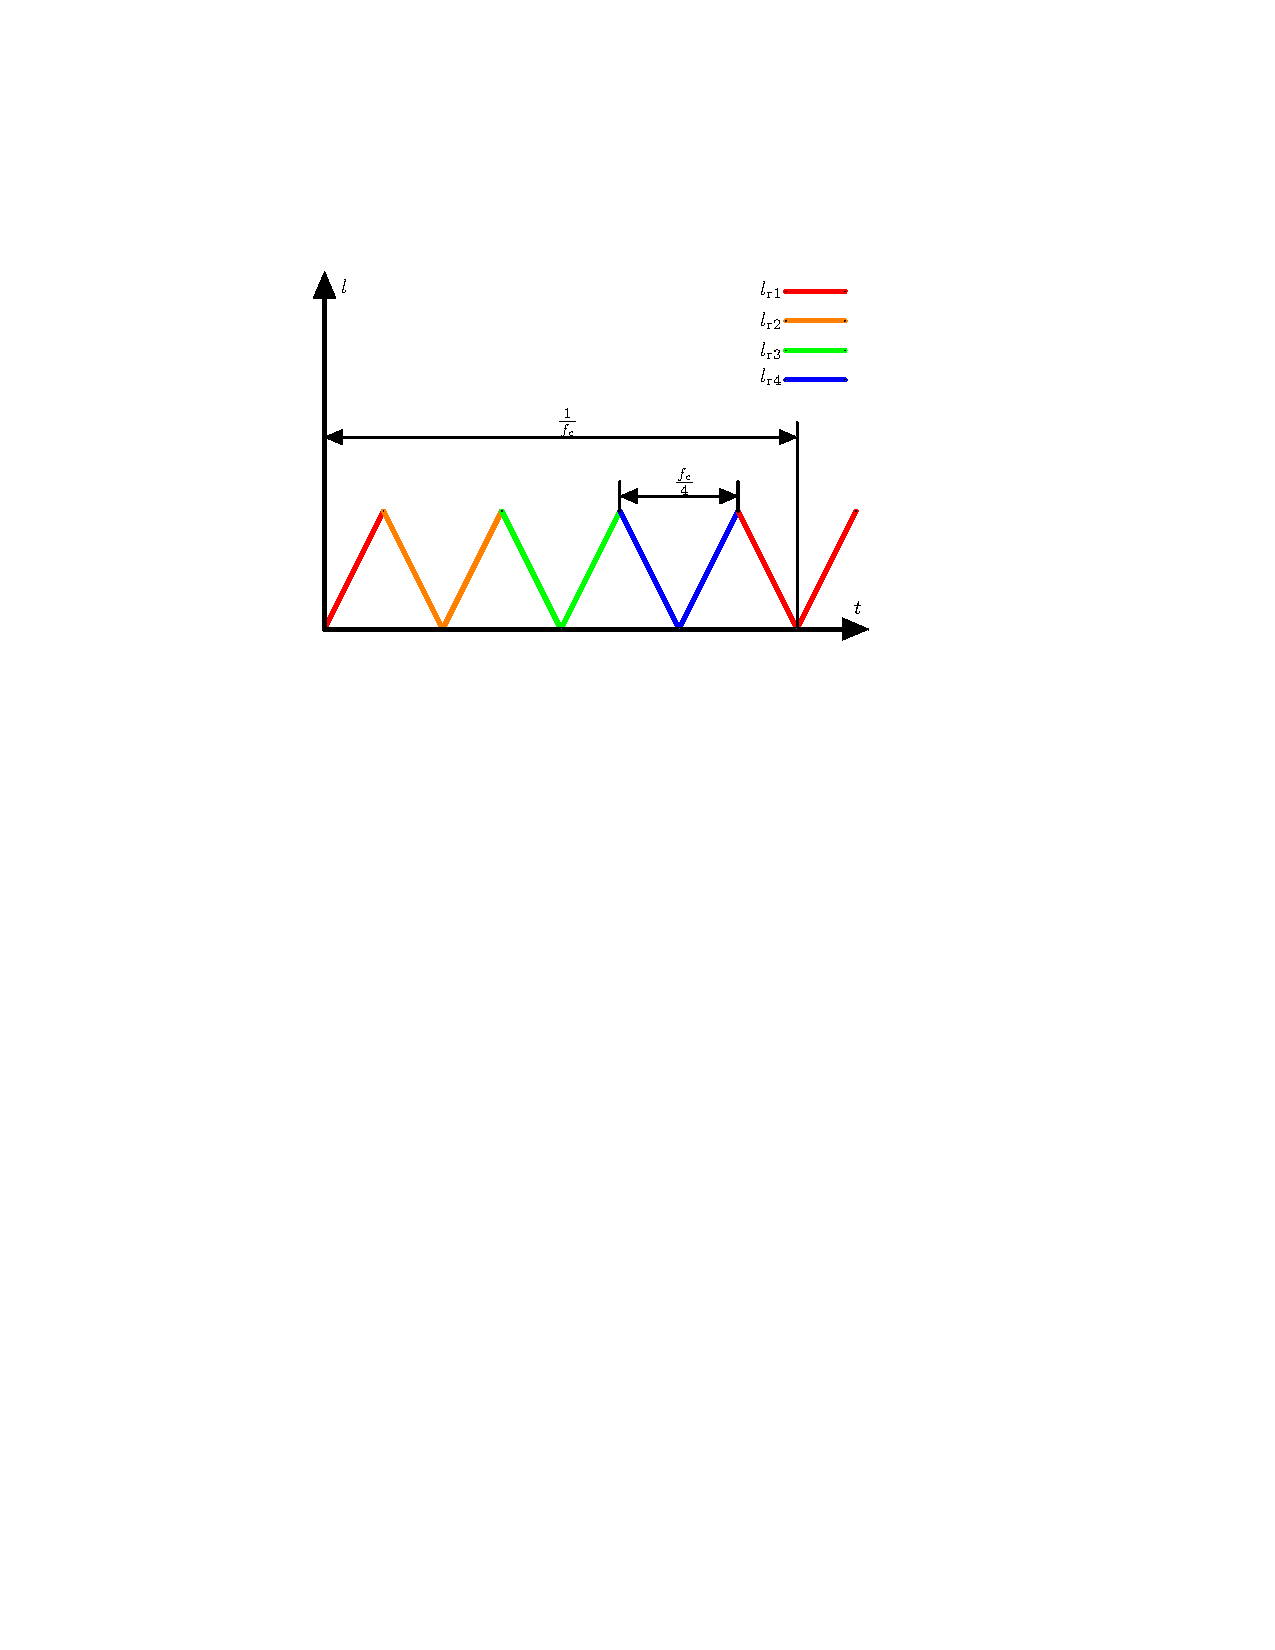
\includegraphics[scale=0.5]{trangle_wave.pdf}
    \caption{Transfer Path 1 length function of time. \textbf{vary the line type for different lengends.Add the transfer effect funciton of time}}
    \label{fig:path_length_trangle_wave}
\end{figure}
\par This attenuation effect with regard to the path length can be characterized as window functions such as Hanning window or Gaussian window \cite{Mark2009}. In this paper, we apply the Gaussian window describing the time-varying transfer path effect,
\begin{equation}
    \sigma(l)=F\exp\left(-\frac{l}{a}\right),\label{eq:general_transfer_path}
\end{equation}
where $l$ is the length of a transfer path, $F$ represents for the strength factor and $a$ is the attenuation factor. $F$ is proportional to the input torque $T_{\rm s}$, here we assume $F=T_{\rm s}/300$. The larger $a$ is, the longer impulses can propagate without a large energy loss. Given Eq. (\ref{eq:path_4_length}) and Eq. (\ref{eq:general_transfer_path}), we can deduce the proportional relationship between path 1 and path 4,
\begin{equation}
    \sigma (l_{{\rm s}i})=F\exp(-\frac{l_{{\rm r}i}+2 R_{\rm p}}{a})=\exp(-\frac{2 R_{\rm p}}{a}) \cdot \sigma(l_{{\rm r}i}).
\end{equation}
For simplicity, we set the $\sigma_i(t)=\sigma\left[l_{{\rm r}i}(t)\right]$ and $\eta=\exp(-\frac{2 R_{\rm p}}{a})$. Fig. \ref{fig:path_length_trangle_wave} shows that $\sigma_{i}(t)$ shifts in time by $(\epsilon_i-\Theta_i)/(2 \pi f_{\rm c})$ relative to $\sigma_1$:
\begin{equation}
    \sigma_{i}(t)=\sigma_{1}(t-\frac{\epsilon_i+\Theta_i}{2 \pi f_{\rm c}}).
\end{equation}
\par Because the transfer path effect function is the exponential function shifting along the time axis with a fixed interval, it can be rewritten as the convolution of exponential function and Dirac comb function with the carrier rotation period $1/f_{\rm c}$.
\begin{equation}
    \sigma_i(t)=\sigma_0(t) \ast \operatorname{III}\left[f_{\rm c} (t - \frac{\epsilon_i+\Theta_i}{2 \pi f_{\rm c}})\right],\label{eq:transfer_path_convolution_form}
\end{equation}
where
\begin{equation}
    \sigma_0(t)=\begin{cases}F \exp(\frac{- 2 \pi R_{\rm r} f_{\rm c} \left|t\right|}{a}),\quad &\frac{-1}{2 M f_{\rm c}} \leq t < \frac{1}{2 M f_{\rm c}}\\
        0, &\text{otherwise}.
    \end{cases}\label{eq:tranfer_path_time_shape}
\end{equation}
\subsection{Natural frequency\label{sec:natural_frequency}}
\par In the above discussion, the gear meshing vibration is simply considered as Dirac impulses. In practice, every impact arising from different components will excite the machine natural frequency. The excited resonance affects the spectral structure globally: the amplitudes of the vibration frequencies around the natural frequency are reinforced and other amplitudes are attenuated. The resonance features a harmonic wave with the amplitude attenuating exponentially, like the vibration of a spring-mass-damper,
\begin{equation}
    \lambda(t)=\begin{cases}
        \exp(-t/\beta)\cdot \sin(2 \pi f_{\rm n} t),\quad & t>=0\\
        0, & t<0
    \end{cases},
\end{equation}
where $\beta>0$ is the structural damping coefficient, $f_{\rm n}$ is the natural frequency.
\par Every time a gear meshing vibration occurs, the machine's natural vibration is excited. This process is mathematically equivalent to the convolution of the impact function of the meshing vibration with the exponentially attenuated harmonic function of the natural vibration. Therefore, considering the effect of the natural vibration, the above signal model can be updated into
\begin{equation}
    \widetilde{x} (t)=\lambda(t) \ast \sum_{i=1}^{M} L_i \sigma_i(t) \left\{ \operatorname{III}\left[f_{\rm m} \cdot (t-\frac{\epsilon_i+\Theta_i}{2 \pi f_{\rm c}})\right]% planet-ring part
    + \eta \operatorname{III}\left[f_{\rm m} \cdot (t + \frac{\epsilon_i+\Theta_i}{2 \pi f_{\rm s}-2 \pi f_{\rm c}}) + \frac{\varphi_i}{2 \pi} \right]% planet-sun part
    \right\},\label{eq:final_signal_model}
\end{equation}
where $\ast$ denotes convolution.
\par For machines with the same configuration, when the load distribution of the planet is uneven, the contact stiffness of the transfer path of each planet inside the planetary gearbox will decrease relative to the case of the uniform load distribution. As a result, The decrease of internal contact stiffness will lead to the decrease of natural frequency of the whole system. Therefore, the variation of the system's natural frequency can be used as a circumstantial evidence to diagnose the load distribution among planets.
\par If the planet pinhole distribute evenly on the carrier, the number of the planets bearing the input load varies as the applied load increases gradually. When the load starts at almost zero, only three planets or one pair of diagonal planets simultaneously engaging with sun and ring gear \cite{Ligata2009}. In this circumstance, load sharing coefficients $L_i=0$ for the unloaded planets. With the ascending input load, another pair of gears get involved. At the same time, the entire transmission system stiffen because more gears support the connection between the input and output. The natural frequency rises along with the system stiffness because the natural frequency equals the square root of stiffness over mass.
\section{Spectral structure \label{sec:spectral_structure}}
\par In this section, we will derive the spectral structure of the above proposed signal model for the in-depth understanding of planetary gearbox vibration. Because natural vibration merely affects the spectral envelope shape, we can consider it separately later on. The gear meshing vibration (Eq. (\ref{eq:planet-ring_meshing}) and Eq. (\ref{eq:planet-sun_meshing})) and transfer path effect arising from the carrier rotation $\sigma_{i}(t)$ are periodic with periods $1/f_{\rm m}$ and $1/f_{\rm c}$, respectively. According to Eq. (\ref{eq:meshing_frequency}) and $f_{\rm r}=0$, $f_{\rm m}=Z_{r} \cdot f_{\rm c}$. Apply Fourier transform to the planet-ring vibration, yields
\begin{equation}
\begin{split}
    \mathcal{F}\left[ \sigma_{{\rm r}i}(t) \xi_{{\rm r}i}(t) \right]=&\mathcal{F}\left\{\sigma_0(t) \ast \operatorname{III}\left[f_{\rm c} \cdot (t - \frac{\epsilon_i+\Theta_i}{2 \pi f_{\rm c}})\right] \cdot A_{{\rm r}i}\operatorname{III}\left[f_{\rm m} \cdot (t-\frac{\epsilon_i+\Theta_i}{2 \pi f_{\rm c}})\right]\right\}\\
    =&A_{{\rm r}i} \cdot \mathcal{F}\left[\sigma_0(t)\right] \cdot \mathcal{F}\left\{\operatorname{III}\left[f_{\rm c} \cdot (t - \frac{\epsilon_i+\Theta_i}{2 \pi f_{\rm c}})\right] \right\}
    \ast \mathcal{F}\left\{ \operatorname{III}\left[f_{\rm m} \cdot (t-\frac{\epsilon_i+\Theta_i}{2 \pi f_{\rm c}})\right] \right\}\\
=&A_{{\rm r}i} \cdot \hat{\sigma}_0(f) \cdot \frac{\operatorname{III}\left(\frac{f}{f_{\rm c}}\right) \exp\left[-\frac{{\rm j} f (\epsilon_i+\Theta_i)}{f_{\rm c}}\right]}{\sqrt{2 \pi} f_{\rm c}} \ast \frac{\operatorname{III}\left(\frac{f}{ Z_{\rm r} f_{\rm c}}\right) \exp\left[-\frac{{\rm j} f (\epsilon_i+\Theta_i)}{ f_{\rm c}}\right]}{\sqrt{2 \pi } Z_{\rm r}f_{\rm c}}\\
=&A_{{\rm r}i} \cdot \frac{\hat{\sigma}_0(f)}{2 \pi Z_{\rm r} f_{\rm c}^{2}} \cdot \sum_{m=-\infty}^{+\infty} \sum_{n=-\infty}^{+\infty} \delta\left[f-(mZ_{\rm r}+n)f_{\rm c}\right] \exp\left[-{\rm j}(m Z_{\rm r}+n)(\epsilon_i+\Theta_i)\right].
\end{split}
\end{equation}
where $\mathcal{F}\{\cdot\}$ denotes Fourier transform, $\hat{\sigma}_0(f)$ is the Fourier spectrum of $\sigma_0(t)$, $\delta\{\cdot\}$ denotes Dirac impulse, $\ast$ denotes convolve. The convolution between two Dirac comb functions equals the summation of all shifted Dirac impulses. Similarly,  the $i$-th planet-sun gear vibration is:
\begin{equation}
    \begin{split}
        \mathcal{F}\left[\sigma_{{\rm s}i}(t) \xi_{{\rm s}i}(t)\right]&=\mathcal{F}\left\{ \eta \cdot \sigma_0(t) \ast \operatorname{III}\left[f_{\rm c}(t-\frac{\epsilon_i+\Theta_i}{2 \pi f_{\rm c}})\right] \cdot A_{{\rm s}i} \operatorname{III} \left[ f_{\rm m} \cdot (t+ \frac{\epsilon_i+\Theta_i}{2\pi f_{\rm s} -2\pi f_{\rm c}} ) +\frac{\varphi_i}{2\pi} \right] \right\}\\
        &=\eta \cdot A_{{\rm s}i} \cdot \mathcal{F}\left[\sigma_0(t)\right] \cdot \mathcal{F}\left\{ \operatorname{III}\left[f_{\rm c} \cdot (t-\frac{\epsilon_i+\Theta_i}{2\pi f_{\rm c}}) \right] \right\} \ast \mathcal{F}\left\{\operatorname{III} \left[ f_{\rm m} \cdot (t+ \frac{\epsilon_i+\Theta_i}{2\pi f_{\rm s} -2\pi f_{\rm c}} ) +\frac{\varphi_i}{2\pi} \right]\right\}\\
        &=\eta \cdot A_{{\rm s}i} \cdot \hat{\sigma}_0(f) \cdot \frac{\operatorname{III}(\frac{f}{f_{\rm c}}) \exp\left[\frac{-{\rm j}f(\epsilon_i+\Theta_i)}{f_{\rm c}}\right]}{\sqrt{2 \pi} f_{\rm c}} \ast \frac{\operatorname{III}(\frac{f}{Z_{\rm r}f_{\rm c}})\exp\left[\frac{{\rm j}f(\epsilon_i+\Theta_i)}{f_{\rm c}-f_{\rm s}}\right] \exp\left(\frac{\varphi_i f}{2\pi Z_{\rm r} f_{\rm c} } \right)}{\sqrt{2 \pi }Z_{\rm r} f_{\rm c}}\\
        &=\eta \cdot A_{{\rm s}i} \cdot \frac{\hat{\sigma}_0(f)}{2 \pi  Z_{\rm r} f_{\rm c}^2} \cdot \sum_{m=-\infty}^{+\infty} \sum_{-\infty}^{+\infty} \delta\left[f-(m Z_{\rm r}+ n)f_{\rm c} \right] \exp\left[ {\rm j} (Z_{\rm s} m - n)(\epsilon_i+\Theta_i) \right] \exp({\rm j}m \varphi_i),
    \end{split}
\end{equation}
where $Z_{\rm s}  (f_{\rm c} -f_{\rm s})= Z_{\rm r} f_{\rm c} =f_{\rm m}$ is applied. Combine the above planet-ring and planet-sun vibration for all planets:
\begin{equation}
    \begin{split}
        X(f) =& \sum_{\rm i=1}^{M} L_i \cdot \left\{\mathcal{F}\left[ \sigma_{{\rm r}i}(t) \xi_{{\rm r}i}(t) \right] + \mathcal{F}\left[\sigma_{{\rm s}i}(t) \xi_{{\rm s}i}(t)\right] \right\}\\
        =&\sum_{\rm i=1}^{M} L_i \cdot \Bigg\{ A_{{\rm r}i} \cdot \frac{\hat{\sigma}_0(f)}{2 \pi Z_{\rm r} f_{\rm c}^{2}} \cdot  \sum_{m=-\infty}^{+\infty} \sum_{n=-\infty}^{+\infty} \delta\left[f-(mZ_{\rm r}+n)f_{\rm c}\right] \exp\left[-{\rm j}(m Z_{\rm r}+n)(\epsilon_i+\Theta_i)\right] 
        \\
        &+\eta \cdot A_{{\rm s}i} \cdot \frac{\hat{\sigma}_0(f)}{2 \pi  Z_{\rm r} f_{\rm c}^2} \cdot \sum_{m=-\infty}^{+\infty} \sum_{-\infty}^{+\infty} \delta\left[f-(m Z_{\rm r}+ n)f_{\rm c} \right] \exp\left[ {\rm j} (Z_{\rm s} m - n)(\epsilon_i+\Theta_i) \right] \exp({\rm j}m\varphi_i) \Bigg\}\\
        =&\frac{\hat{\sigma}_0(f)}{2\pi Z_{\rm r} f_{\rm c}^{2}} \sum_{m=-\infty}^{+\infty} \sum_{n=-\infty}^{+\infty} \delta\left[f-(m Z_{\rm r}+n) f_{\rm c} \right] \Bigg\{ \sum_{i=1}^{M} L_i \cdot A_{{\rm r}i} \cdot \exp\left[ -{\rm j}(m Z_{\rm r}+n)(\epsilon_i+\Theta_i)\right]\\
        &+\eta \cdot L_i \cdot A_{{\rm s}i} \cdot \exp({\rm j}m\varphi_i) \cdot\exp\left[{\rm j}(m Z_{\rm r}-n)(\epsilon_i+\Theta_i) \right] \Bigg\}.
    \end{split}
\end{equation}
\par We assume the isotropy of planet and the amplitudes of $i$-th planet gear meshing impacts $A_{{\rm r}i}$ and $A_{{\rm s}i}$ remain the same for every planet, that is $A_{{\rm r}i}=A_{{\rm r}1}$, $A_{{\rm s}i}=A_{{\rm s}1} $. When all planets locate at the nominal positions ($\epsilon_i=0$), each planet bears the same torque ($L_i=L_1$), The $X(f)$ in the ‘perfect’ case is
\begin{equation}
    \begin{align}
        X(f)=\frac{L_1 \cdot \hat{\sigma}_0(f)}{2\pi Z_{\rm r} f_{\rm c}^{2}} \sum_{m=-\infty}^{+\infty} \sum_{n=-\infty}^{+\infty} \delta\left[f-(m Z_{\rm r}+n) f_{\rm c} \right] 
              \Bigg\{ \sum_{i=1}^{M}  A_{{\rm r}1}  \exp\left[ -{\rm j}(m Z_{\rm r}+n)\Theta_i\right]\\
              +\eta A_{{\rm s}1}\exp({\rm j}m\varphi_i) \exp\left[{\rm j}(m Z_{\rm r}-n)\Theta_i \right]\Bigg\}
    \end{align},%planet-sun part
\end{equation}
where
\begin{equation}
        \sum_{i=1}^{M} \exp[-{\rm j} (m Z_{\rm r} + n)\Theta_i]=\sum_{i=1}^{M} \exp[-{\rm j}(m Z_{\rm r}+n)\frac{2 \pi (i-1)}{M}]=\begin{cases}
            M, \quad \frac{m Z_{\rm r}+n}{M} \in \mathbb{N}\\
            0, \quad \frac{m Z_{\rm r}+n}{M} \notin \mathbb{N}
        \end{cases},\label{eq:carrier_harmonic_ring}
\end{equation}
\begin{equation}
    \sum_{i=1}^{M} \exp[{\rm j} (m Z_{\rm s} - n)\Theta_i]=\sum_{i=1}^{M} \exp[{\rm j}(m Z_{\rm s}-n)\frac{2 \pi (i-1)}{M}]=\begin{cases}
         M, \quad \frac{m Z_{\rm s}-n}{M} \in \mathbb{N}\\
        0, \quad \frac{m Z_{\rm s}-n}{M} \notin \mathbb{N}
    \end{cases}.\label{eq:carrier_harmonic_sun}
\end{equation}
\par According to the above Eq. (\ref{eq:carrier_harmonic_ring}) and Eq. (\ref{eq:carrier_harmonic_sun}), when $(m Z_{\rm s}-n)$ or $(m Z_{\rm s}-n)$ is the multiple of planet number $M$, the corresponding Fourier coefficient is nonzero. The carrier harmonics only peak at the multiple of planet number $M$ when planet distributes evenly. Interestingly, all planet distributes evenly ($\epsilon_i=0$) can only be achieved when the condition $(Z_{\rm r}+Z_{\rm s})/M \in \mathbb{N}$ is guaranteed (explanations see \nameref{Appendix}). Therefore, $(m Z_{\rm r}+n)/M$ and $(m Z_{\rm s}-n)/M$ will be integers at one time. 
\par When $\epsilon_i \neq 0$, all carrier harmonic $(m Z_{\rm r} + n)$ and $(m Z_{\rm s} - n)$ will appear with their amplitude arising from planet-ring meshing ($\sum_{i=1}^{M} L_i \exp[-{\rm j} (m Z_{\rm r} + n)(\epsilon_i+\Theta_i)]$) and planet-sun meshing ($\sum_{i=1}^{M} L_i \exp[-{\rm j} (m Z_{\rm s} - n)(\epsilon_i+\Theta_i)]$), respectively. For example, the second planet carries all load (the $L_2=1$ and $L_i=0,i\neq2$), the $(m Z_{\rm r} + n)$ order harmonic manifests itself with the amplitude of $\sum_{i=1}^{M} L_i \exp[-{\rm j} (m Z_{\rm r} + n)(\epsilon_i+\Theta_i)]$, which is nonzero. The amplitudes of the planet number multiples of carrier harmonics scale down to $\exp[{\rm j}(m Z_{\rm r}+n)\epsilon_i]$ and $\exp[{\rm j}(m Z_{\rm s}-n)\epsilon_i]$, respectively.
\par Natural vibration further scales the amplitude of spectral components. Apply the convolution theorem to the signal model considering natural vibration (Eq. (\ref{eq:final_signal_model})), the final version of spectrum:
\begin{equation}
        \widetilde{X}(f)= \mathcal{F}\left[\lambda(t) \ast x(t) \right]
                    = \mathcal{F}\left[\lambda(t)\right] \cdot \mathcal{F}\left[x(t)\right]
                    = \hat{\lambda}(f) \cdot \widetilde{X}(f)
\end{equation}
where $\hat{\lambda}(f)$ is the Fourier transform of $\lambda(t)$:
\begin{equation}
    \hat{\lambda}(f)=\frac{\sqrt{2 \pi } \beta ^2 f_{\rm n}}{-4 \pi ^2 \beta ^2 f^2  + 4 \pi ^2 \beta ^2 f_{\rm n}^2+1 - {\rm j} 4 \pi  \beta  f}
\end{equation}
%%%%%%%%%%%%%%%%%%%%%%%% Numerical simulation %%%%%%%%%%%%%%%%%%%%%%%
\section{Discussion on model factors\label{sec:factor_discussion}}
\par We use MATLAB\textsuperscript \textregistered \ to simulate the proposed signal model. To validate the generality of the propose model, we take different planet pinhole position errors, planet numbers and input torques into account. The simulation parameters are listed in Table \ref{}.
\par In general, if the planet locates the nominal position, only the planet number multiples of carrier harmonics appear (give more specific results in figures), which accords with the Eq. (\ref{eq:carrier_harmonic_ring}) and Eq. (\ref{eq:carrier_harmonic_sun}). When the planet center deviates from the nominal position, other carrier orders emerges. Differing from the conclusion in \cite{Mark2009}, the dominant planet number multiple peaks do not shrink too, because we also consider the phase modulation induced by the pinhole position errors. 
\par Fig. \ref{fig:Shifted_natural_frequency} explain the mechanism of shifted natural frequency -- the resonance frequency shift from 300Hz to 400Hz. With the limited measurement conditions about natural frequency in industrial applications, the above natural frequency shift can only be validated qualitatively. The signal model in Eq. (\ref{eq:final_signal_model}) indicates the natural frequency affects the spectral envelope shape. As the load increases, the envelope peak shifting to a higher frequency signifies the unequal load sharing among planets. 

\begin{figure}[pos=htbp]
    \centering
    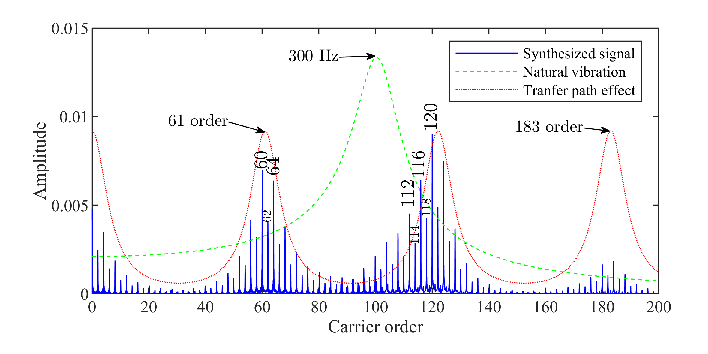
\includegraphics[scale=1]{Shifted_natural_frequency}
    \caption{Spectral summit cluster shifts towards a lower frequency due to the uneven load distribution of planets}\label{fig:Shifted_natural_frequency}
\end{figure}
\par The extra sidebands at non M multiples of carrier orders can be attributed by the phase modulation effects (with a period of carrier rotation period and fluctuates at each planet position (both time and space)).
\par The amplitude envelope sharpe can also evidence the existence of planet position shifts. Because the support stiffness weakens, the resonance frequency of the entire system shift towards the y-axis. Fig. \ref{fig:overview_normal_fourier} and Fig. \ref{fig:Shifted_natural_frequency} show the resonance frequency shift from 300Hz to 400Hz.
\subsection{Different planet numbers}
\par When at least one central members can float along the radial direction, three planets can offset the influence of uneven load distribution arising from limited pinhole position errors. The condition of floating central members can be satisfied commonly, because the manufacturers deliberately design separable sun gears  and flexible couplings.  When tangential error in planet pinhole occur, the time shifts to the transfer path effects still make the impulsive intervals between adjacent planets uniform. Fig \ref{fig:simulated_p3}(b) present the quasi phase modulation -- if we regard all planets as one -- in time domain.  The corresponding spectrum also manifests the non planet number ($M=3$) peaks. In the baseline case where these pinhole errors are absent, the carrier orders merely appear at the multiples of three.
\begin{figure}[pos=htbp]
    \centering
    (a) 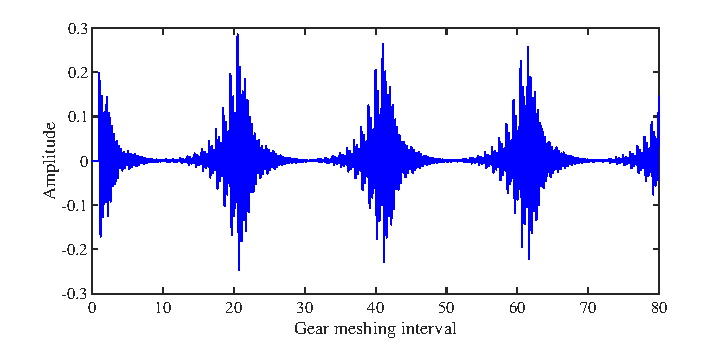
\includegraphics[scale=\myscale,valign=t]{Time_p3_normal.pdf}
    (b) 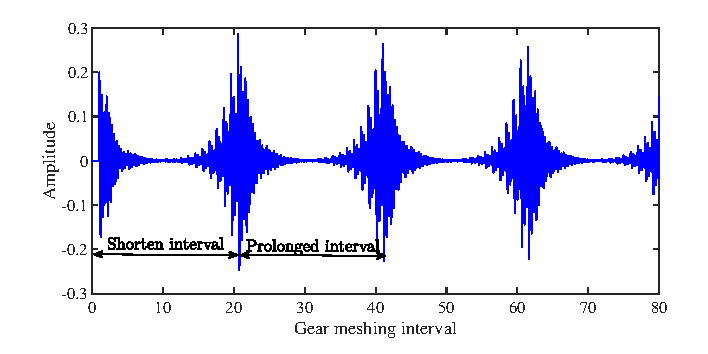
\includegraphics[scale=\myscale,valign=t]{Time_p3_fault.pdf}\\
    \hspace*{1.5em}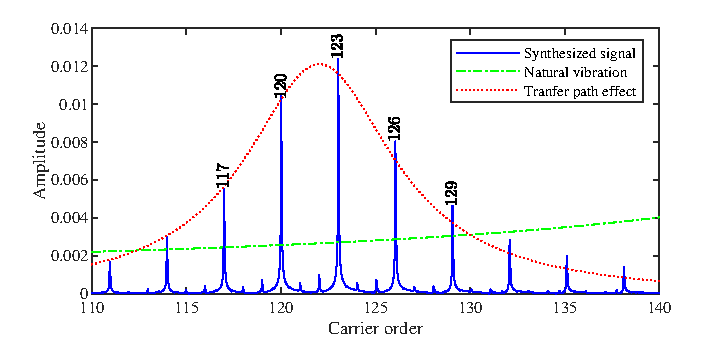
\includegraphics[scale=\myscale,valign=t]{Freq_p3_normal.pdf}
    \hspace*{1.5em}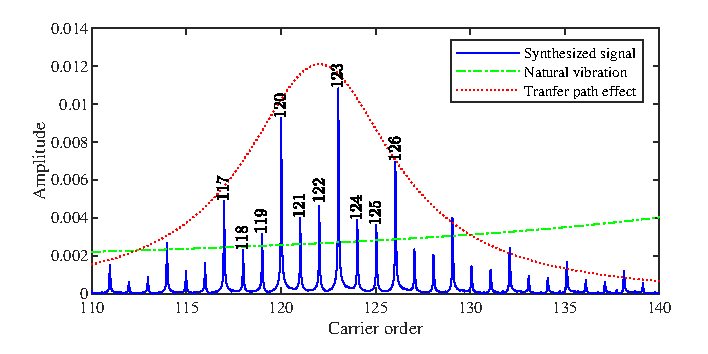
\includegraphics[scale=\myscale,valign=t]{Freq_p3_fault.pdf}
    \caption{Simulated signals of planetary boxes of 3 planets: (a) normal case; (b) $0.5^\circ$ position error on second planet pinhole.}
    \label{fig:simulated_p3}
\end{figure}
\par In cases where planet number $M\geq4$, floating members in planetary gearboxes cannot neutralize all effects on load sharing conditions caused by planet pinhole position errors. The time domain signals in Fig. \ref{fig:simulated_p4}(b) ($M=4$) demonstrates the  pinhole errors modulates the  timing and strength of  each planet impulse at the same time. Shown in the Fourier spectra of fault cases, the quasi amplitude and frequency modulation gives rise to the extra sidebands emerge at the non M multiples. While carrier orders only peak with the intervals of  planet number in Fig. \ref{fig:simulated_p4}(a) ($M=4$).
\begin{figure}[pos=htbp]
    \centering
    (a) 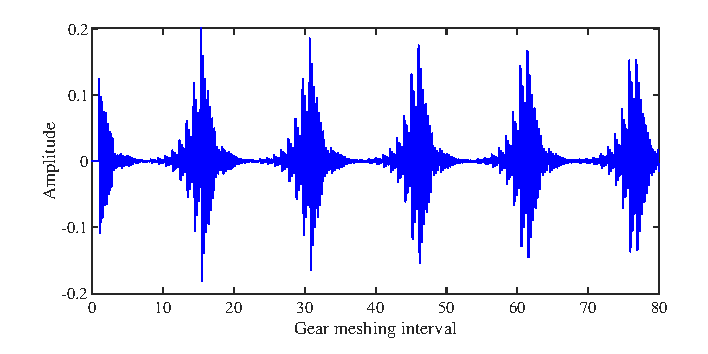
\includegraphics[scale=\myscale,valign=t]{Time_p4_normal.pdf}
    (b) 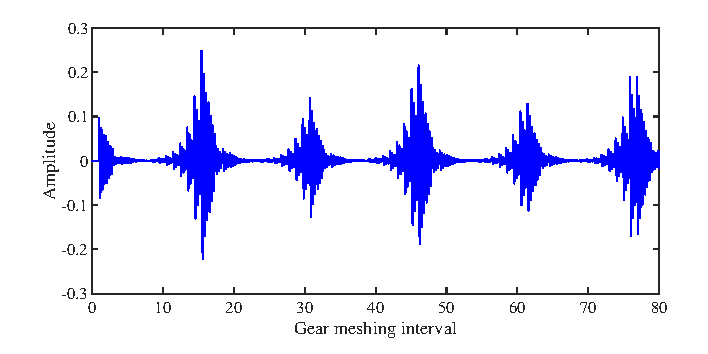
\includegraphics[scale=\myscale,valign=t]{Time_p4_fault.pdf}\\
    \hspace*{1.5em}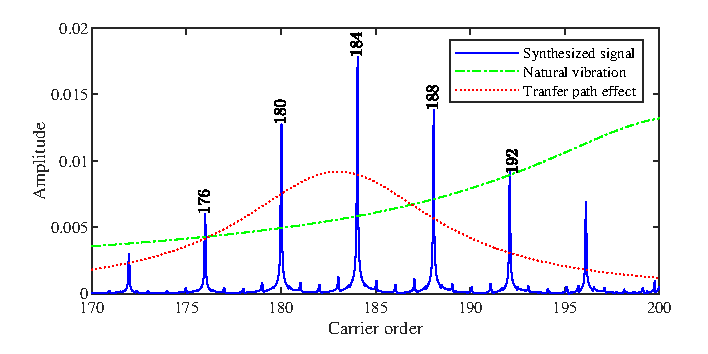
\includegraphics[scale=\myscale,valign=t]{Freq_p4_normal.pdf}
    \hspace*{1.5em}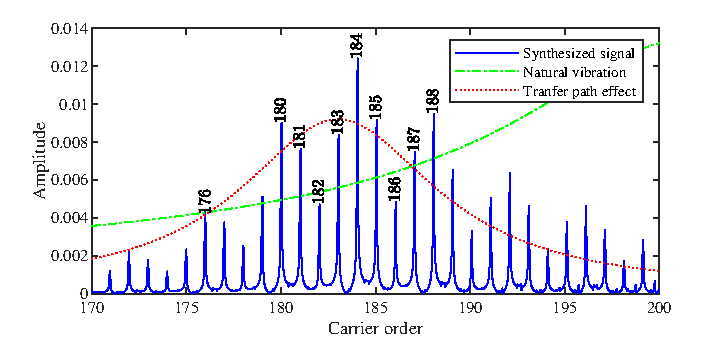
\includegraphics[scale=\myscale,valign=t]{Freq_p4_fault.pdf}
    \caption{Simulated signals of planetary boxes of 4 planets: (a) normal case; (b) $0.5^\circ$ position error on second planet pinhole.}
    \label{fig:simulated_p4}
\end{figure}
\subsection{Effects of input torque}
\par As explained in the Section \ref{sec:transfer_path}, the input torque affects the impulsive strengths of planets contacting with sun and ring gears, so as to scale the whole signal amplitudes. Fig. \ref{fig:simulated_p5_normal} shows that the larger input torque is applied, the higher signal amplitude in both time and frequency domains. 
\par The input torque also affects the numbers of contacting planets. As the input torque increases from a lower value, more planets get involved in bearing load gradually. Thus, the natural frequency of the system rises. Fig. \ref{fig:simulated_p5_fault} presents the natural frequency shifts in spectrum. In addition, the larger input torque can improve load sharing conditions to be more uniform. Extra non M multiples shrinks relatively to the dominant M multiples. 
\begin{figure}[pos=htbp]
    \centering
    (a) 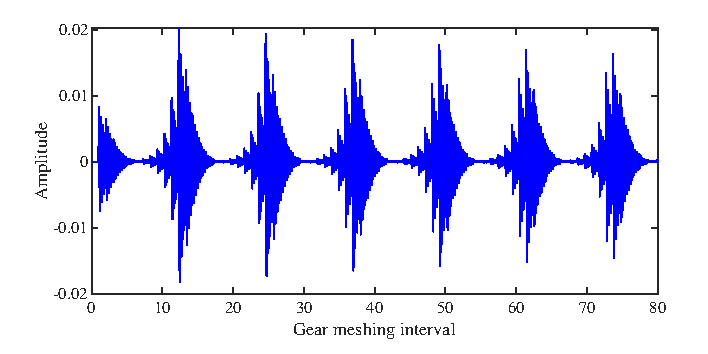
\includegraphics[scale=\myscale,valign=t]{Time_p5_normal_L30.pdf}
    (b) 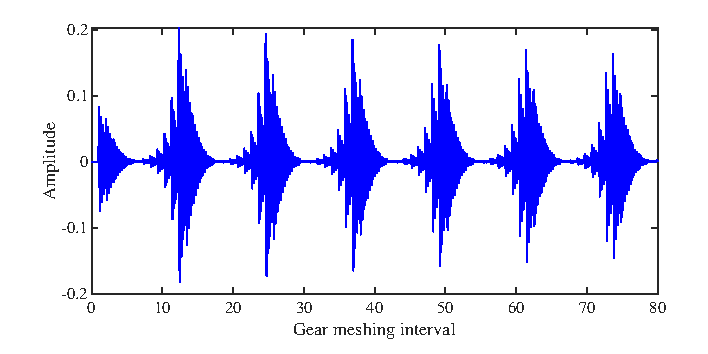
\includegraphics[scale=\myscale,valign=t]{Time_p5_normal_L300.pdf}\\
    \hspace*{1.5em}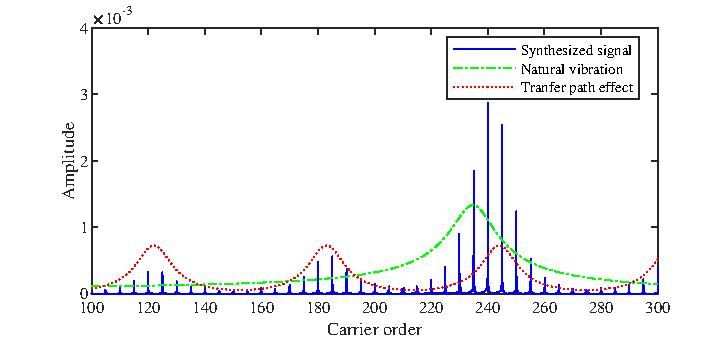
\includegraphics[scale=\myscale,valign=t]{Freq_p5_normal_L30.pdf}
    \hspace*{1.5em}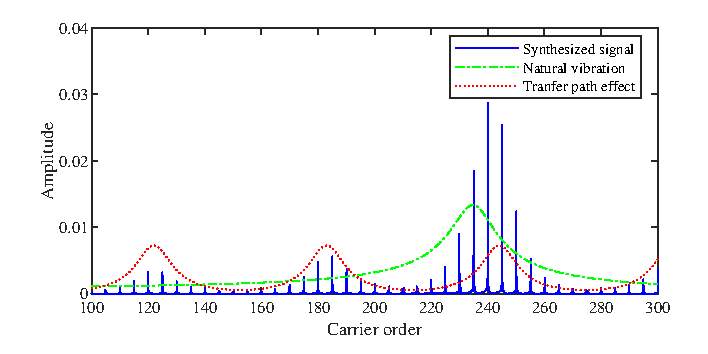
\includegraphics[scale=\myscale,valign=t]{Freq_p5_normal_L300.pdf}
    \caption{Simulated signals of normal planetary boxes with different input torques: (a) $T_{\rm s}=30\ {\rm N\ m}$; (b) $T_{\rm s}=300\ {\rm N\ m}$.}
    \label{fig:simulated_p5_normal}
\end{figure}
\begin{figure}[pos=htbp]
    \centering
    (a) 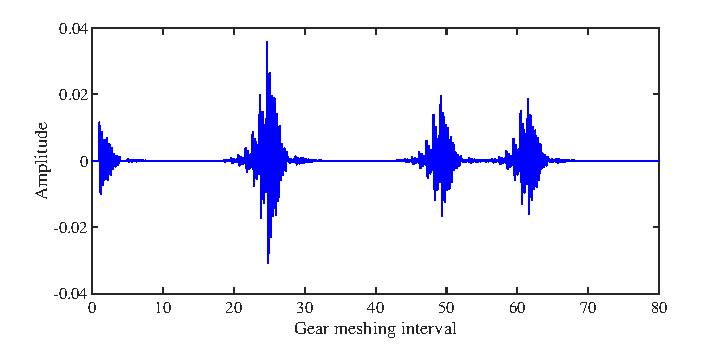
\includegraphics[scale=\myscale,valign=t]{Time_p5_fault_L30.pdf}
    (b) 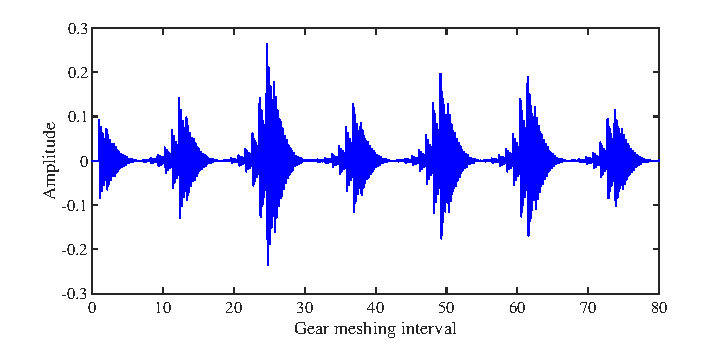
\includegraphics[scale=\myscale,valign=t]{Time_p5_fault_L300.pdf}\\
    \hspace*{1.5em}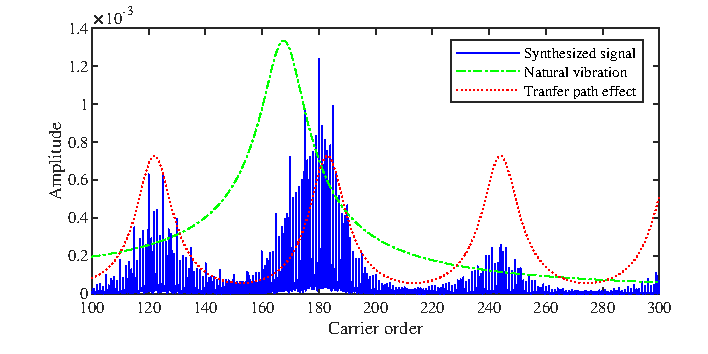
\includegraphics[scale=\myscale,valign=t]{Freq_p5_fault_L30.pdf}
    \hspace*{1.5em}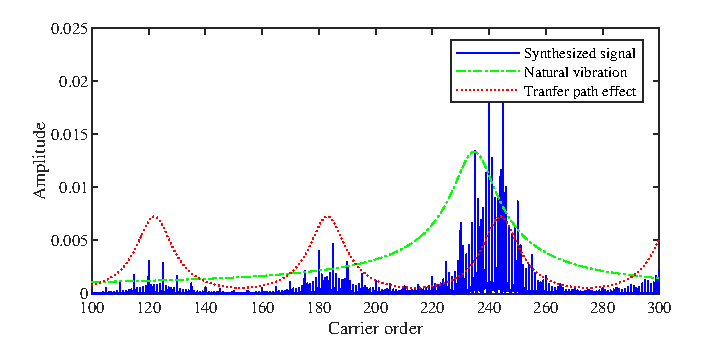
\includegraphics[scale=\myscale,valign=t]{Freq_p5_fault_L300.pdf}
    \caption{Simulated signals of faulty planetary boxes with $0.4^\circ$ error in the third planet pinhole and different input torques: (a) $T_{\rm s}=30\ {\rm N\ m}$; (b) $T_{\rm s}=300\ {\rm N\ m}$;.}
    \label{fig:simulated_p5_fault}
\end{figure}
\subsection{Severity levels of pinhole error}
\par The severity of pinhole error mainly influences the signal spectra in two stages. At the beginning the planetary gearbox is free of pinhole errors. All planets bear the load evenly with the same strength as shown in time domain of Fig. \ref{fig:simulated_p6_normal}(a), and peaks only exist at the multiples of planet number ($M=6$). When a slight error ($0.1^\circ$ on the fourth planet pinhole) occurs, Fig. \ref{fig:simulated_p6_severity}(b) demonstrates the non M multiples of carrier orders emerge in spectrum.  At the first stage, an increasing error level ($1^\circ$) leads to the amplified the components of non M multiples clustering around the dominant peaks, as presented in Fig. \ref{fig: simulated_p6_severtiy}(c). At the second stage, if we continually enlarges the error to $2.1^\circ$, a pair of planets will separate from contact and the location of envelope summit along with the system natural frequency will decrease to a lower range. Fig. \ref{fig:simulated_p6_severity}(d) illustrates this phenomenon.
\begin{figure}[pos=htbp]
    \centering
    (a) 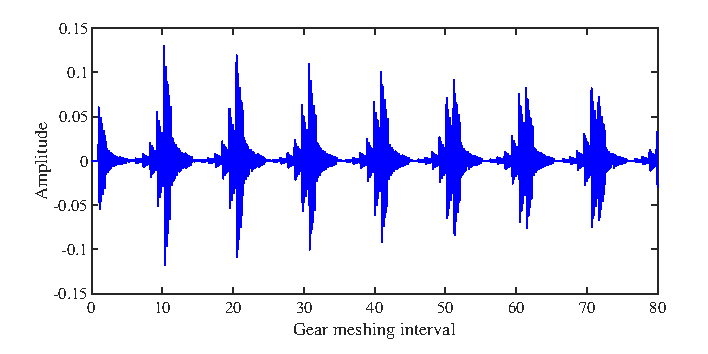
\includegraphics[scale=\myscale,valign=t]{Time_p6_normal.pdf}
    (b) 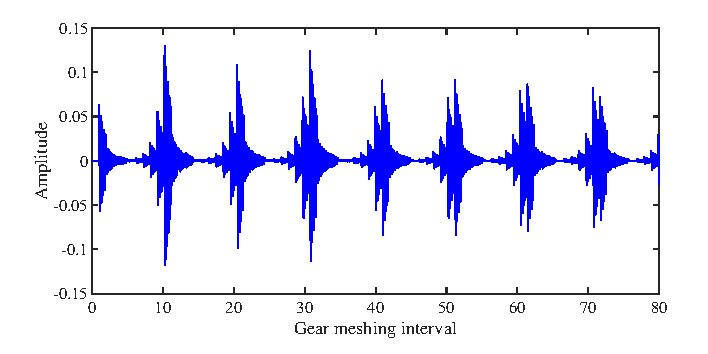
\includegraphics[scale=\myscale,valign=t]{Time_p6_slight_error.pdf}\\
    \hspace*{1.5em}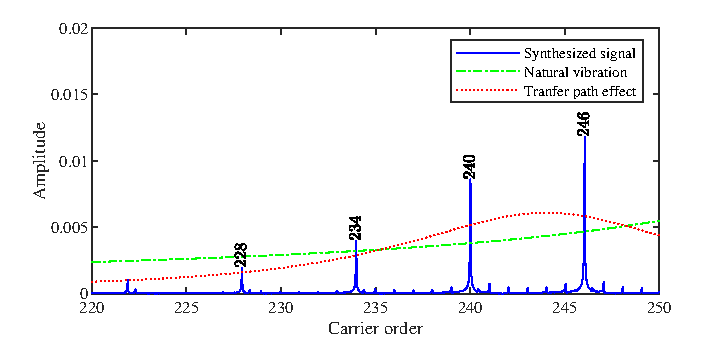
\includegraphics[scale=\myscale,valign=t]{Freq_p6_normal.pdf}
    \hspace*{1.5em}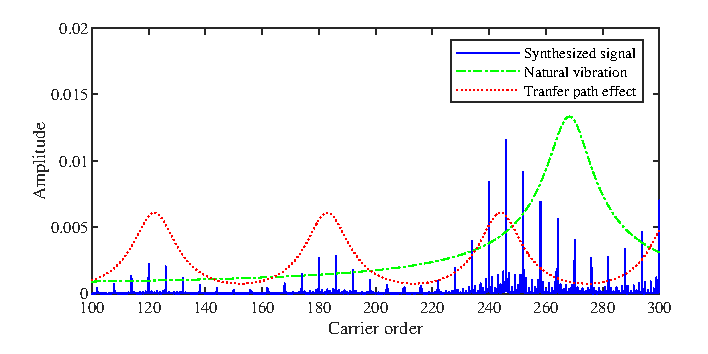
\includegraphics[scale=\myscale,valign=t]{Freq_p6_slight_error.pdf}\\
    (c) 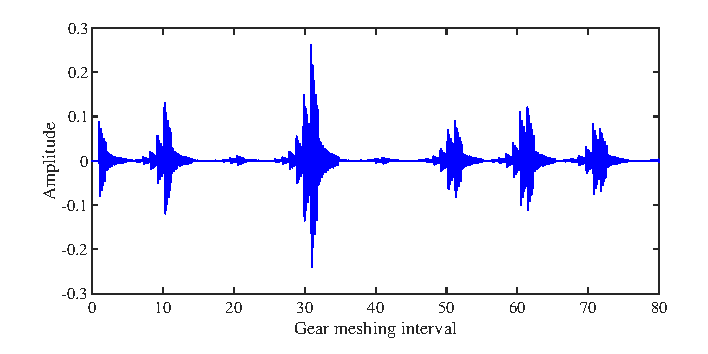
\includegraphics[scale=\myscale,valign=t]{Time_p6_medium_error.pdf}
    (d) 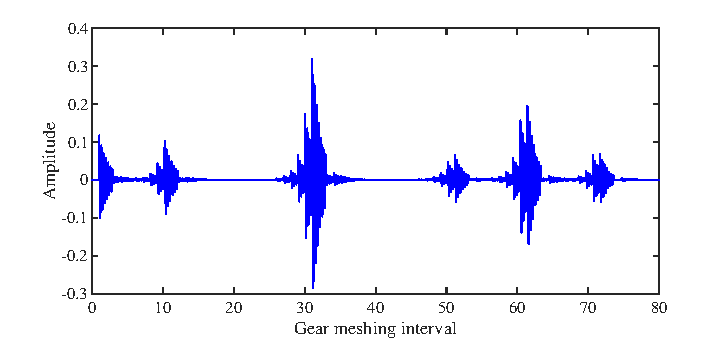
\includegraphics[scale=\myscale,valign=t]{Time_p6_severe_error.pdf}\\
    \hspace*{1.5em}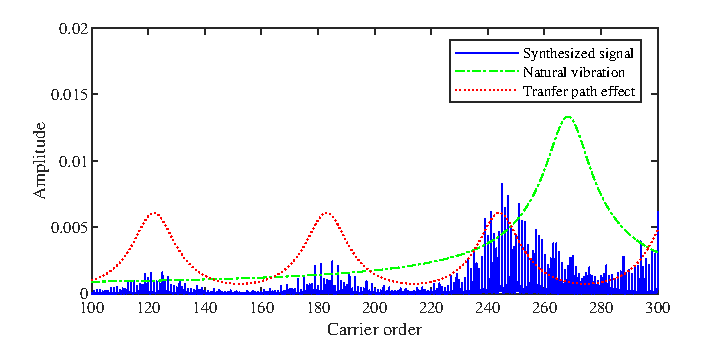
\includegraphics[scale=\myscale,valign=t]{Freq_p6_medium_error.pdf}
    \hspace*{1.5em}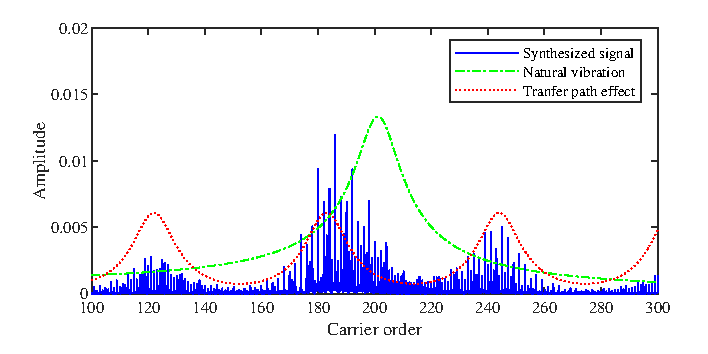
\includegraphics[scale=\myscale,valign=t]{Freq_p6_severe_error.pdf}
    \caption{Simulated signals of planetary boxes with errors on the fourth planet in various severity levels: (a) normal; (b) $0.1^\circ$; (c) $1^\circ$; (d) $2.1^\circ$.}
    \label{fig:simulated_p6_severity}
\end{figure}
\section{Experimental validation\label{sec:experimental_validation}}
We implemented experiments to substantiate the proposed signal model and the above theoretical derivation.
\subsection{Experimental settings}
\par We set up a test rig consisting of a motor, a planetary gearbox, an encoder,  a torque transducer and a generator as load, as shown in Fig. \ref{fig:test_rig}. Besides a normal planetary gearbox with four planets as baseline,  we designed a fault case where one planet pinhole ahead of the nominal position by $0.1^{\circ}$, demonstrated in Fig. \ref{fig:exp_pinhole_error}. The rated parameters and configuration parameters of the planetary gearbox are listed in Table \ref{tab:rated_parameters} and Table \ref{tab:configuration_parameters}, respectively. The sampling frequency of the acquisition system is $20480$ Hz, and the duration is $60$ s. The rotating frequency of sun gear is $8.45$ Hz. $30$ N m load is applied. The gear meshing frequency is $f_{\rm m}=228.15$ Hz and carrier frequency is $f_{\rm c}=2.1125$ Hz.
\begin{figure}[pos=htbp]
    \centering
    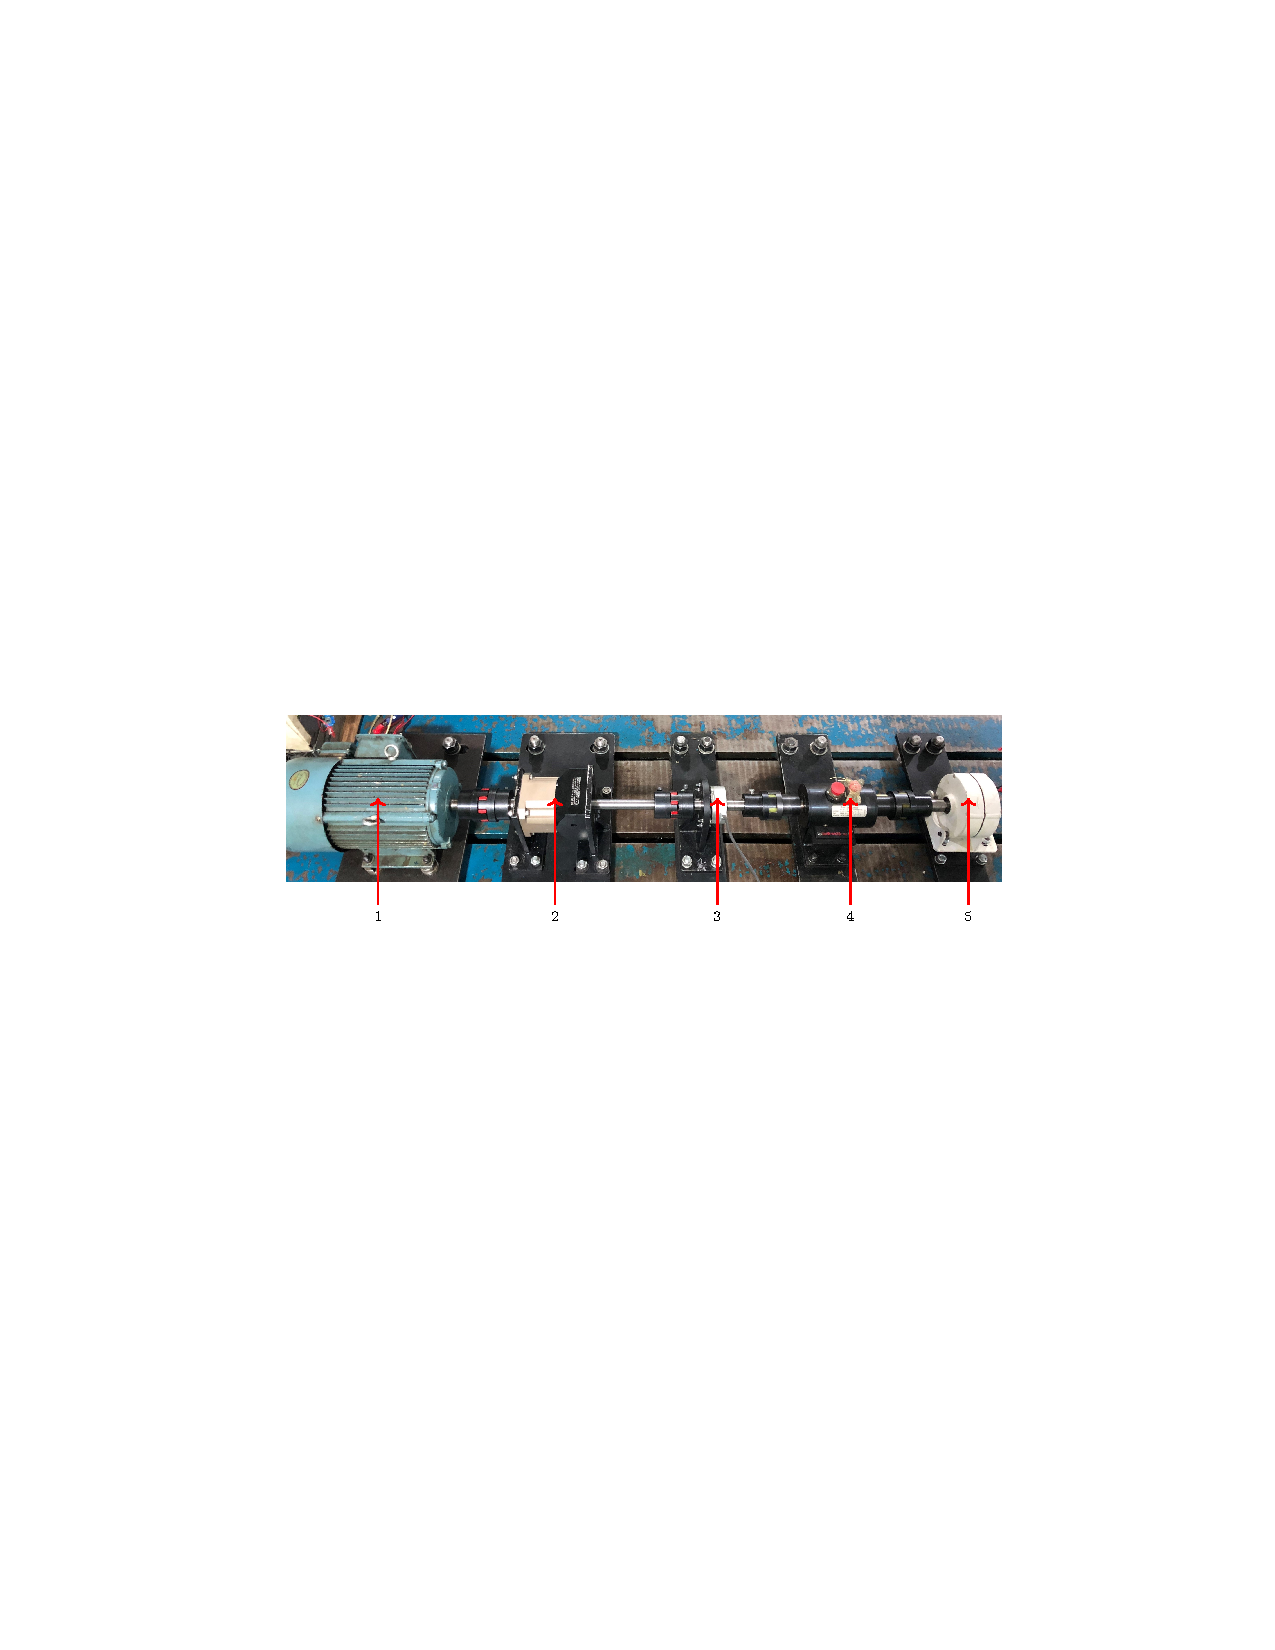
\includegraphics{test_rig_configuration.pdf}
    \caption{Planetary gearbox test rig: 1. induction motor; 2. planetary gearbox; 3. rotary encoder; 4. torque transducer and 5. generator.}
    \label{fig:tets_rig}
\end{figure} 
\begin{figure}[pos=htbp]
    \centering
    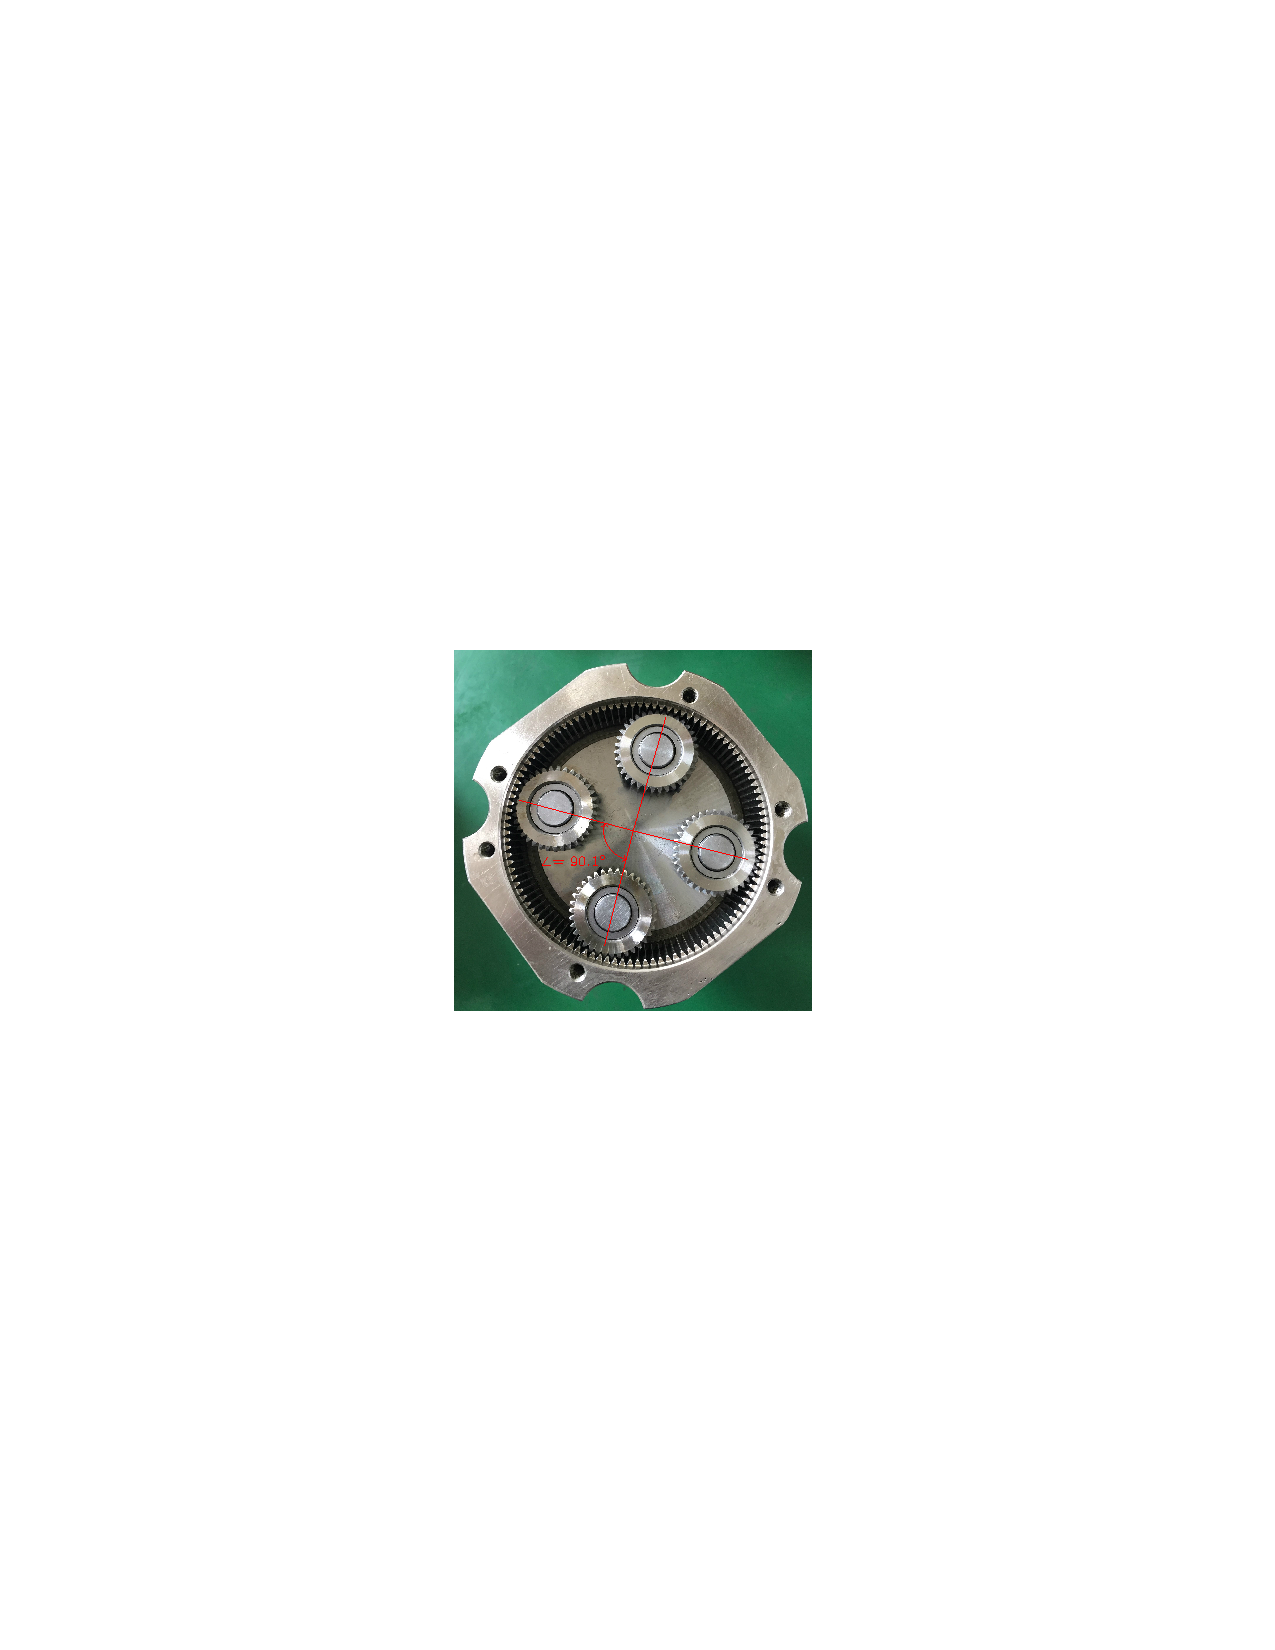
\includegraphics[scale=0.7]{exp_pinhole_error.pdf}
    \caption{Planetary gearbox with a pinhole position error}
    \label{fig:exp_pinhole_error}
\end{figure}
%%%%%%%%%%%%%%%%%%%%%%% rated parameters %%%%%%%%%%%%%%%%%%%%%%%
\begin{table}
    \centering
    \caption{Rated parameters of planetary gearbox.\label{tab:rated_parameters}}
    \begin{tabular}{*{3}{>{\centering\arraybackslash}m{10em}}}
    \toprule
    Power (kW) &  Speed (rpm) & Speed ratio \\
    \midrule
    8 & 1500 &  4 \\
    \bottomrule
    \end{tabular}
    \end{table}
%%%%%%%%%%%%%%%%%%%%%%% gearbox configuration %%%%%%%%%%%%%%%%%
\begin{table}
\centering
\caption{Confiuration parameters of planetary gearbox.\label{tab:configuration_parameters}}
\begin{tabular}{*{4}{>{\centering\arraybackslash}m{8em}}}
\toprule
Gear & Sun gear & Planet (number) & Ring gear\\
\midrule
Number of teeth & 36 & 35 (3) &  108 \\
\bottomrule
\end{tabular}
\end{table}
\subsection{Experimental data analysis}
\par Fig. \ref{fig:exp_natural_frequency_shift} overviews the spectra of normal and fault cases. Generally, the natural vibration and transfer path effects jointly shape the envelopes of the normal and fault spectra. By contrast, the envelope summit of normal spectrum locates at the higher frequency range than the fault case since the natural frequency of normal case is higher. This indicates that the pinhole position error can cause planets to disconnect with sun or ring gears, verifying the natural frequency shift described in Section \ref{sec:natural_frequency}.
\begin{figure}[pos=htbp]
    \centering
    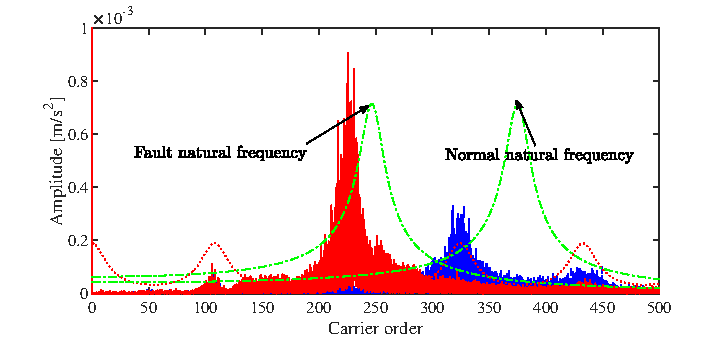
\includegraphics{Exp_natural_frequency_shift.pdf}
    \caption{Spectrum overview of experimental data}
    \label{fig:exp_natural_frequency_shift}
\end{figure}
\par The signal of unequal load sharing displays more irregular impulses within one carrier rotation period, demonstrated in Fig. \ref{fig:exp_time_freq_comparison}(b). While the impulsive amplitudes and intervals are more evenly distributed in the normal case (Fig. \ref{fig:}(a)). By comparison between frequency domains, non M multiples of carrier order peaks clearly in the fault case, evidencing the non-uniform load distribution among planets. The unconspicuous noise components are attributed to the inevitable errors during manufacturing and assembling.
\begin{figure}[pos=htbp]
    \centering
    (a) 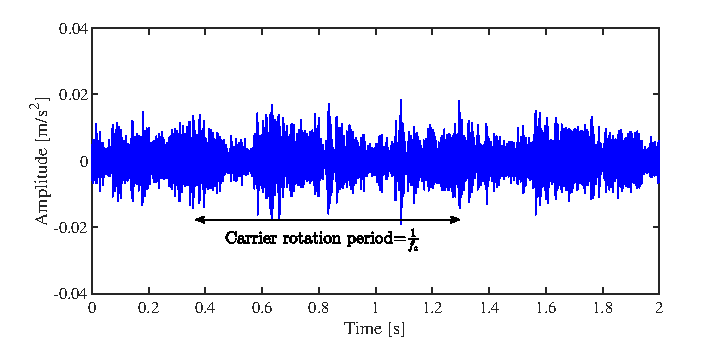
\includegraphics[scale=\myscale,valign=t]{Exp_Time_normal.pdf}
    (b) 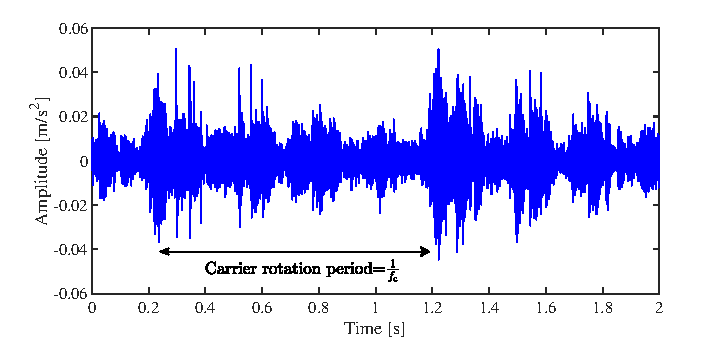
\includegraphics[scale=\myscale,valign=t]{Exp_Time_fault.pdf}\\
    \hspace*{1.5em}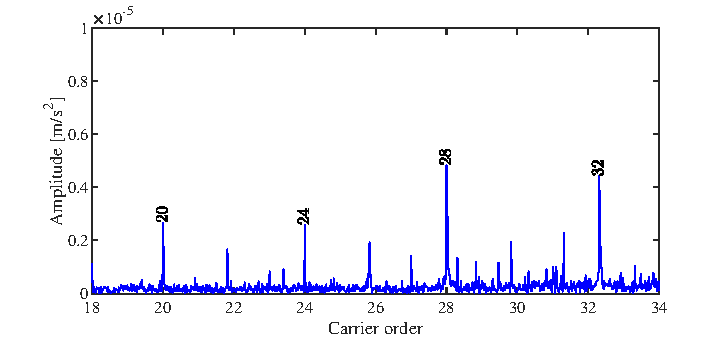
\includegraphics[scale=\myscale,valign=t]{Exp_normal_22.pdf}
    \hspace*{1.5em}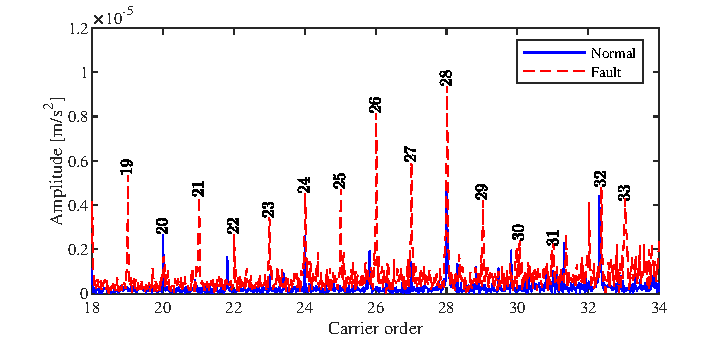
\includegraphics[scale=\myscale,valign=t]{Exp_fault_22.pdf}
    \caption{Experimental data analysis in time and frequency domains: (a) normal case; (b) fault case.}
    \label{fig:exp_time_freq_comparison}
\end{figure}
\section{Conclusions \label{sec:conclusions}}
\par We established a vibration signal model of planetary gearboxes and derived the corresponding Fourier spectrum, considering the effects of transfer path, gear meshing vibration, natural vibration, amount of contacting planets and load sharing among planets. Only planet number multiples of carrier rotating frequency appear in the Fourier spectrum of the normal case, while the spectrum of unequal load sharing signal additionally presents non planet number multiples of carrier rotating frequency. The pinhole position error severity and the input torque jointly affect the load sharing conditions, the number of contacting planets and the system natural frequency. With the increasing pinhole error severity or the decreasing applied input torque, fewer planets bear loads, the stiffness of the whole system decreases, the natural frequency shifts towards a lower range and the load sharing conditions deteriorate. Thus, the additional carrier orders and the shifted natural frequency in the spectrum can evidence the unequal load sharing among planets for diagnostic purposes. In the future, we will investigate the modeling of unequal load sharing among planets with the existence of gear and bearing faults.
%%%%%%%%%%%%%%%%%%%%%%%%%%%%%% Appendix %%%%%%%%%%%%%%%%%%%%%%%%%%%%%
\section*{Appendix\label{Appendix}}
\begin{figure}[pos=htbp]
    \centering
    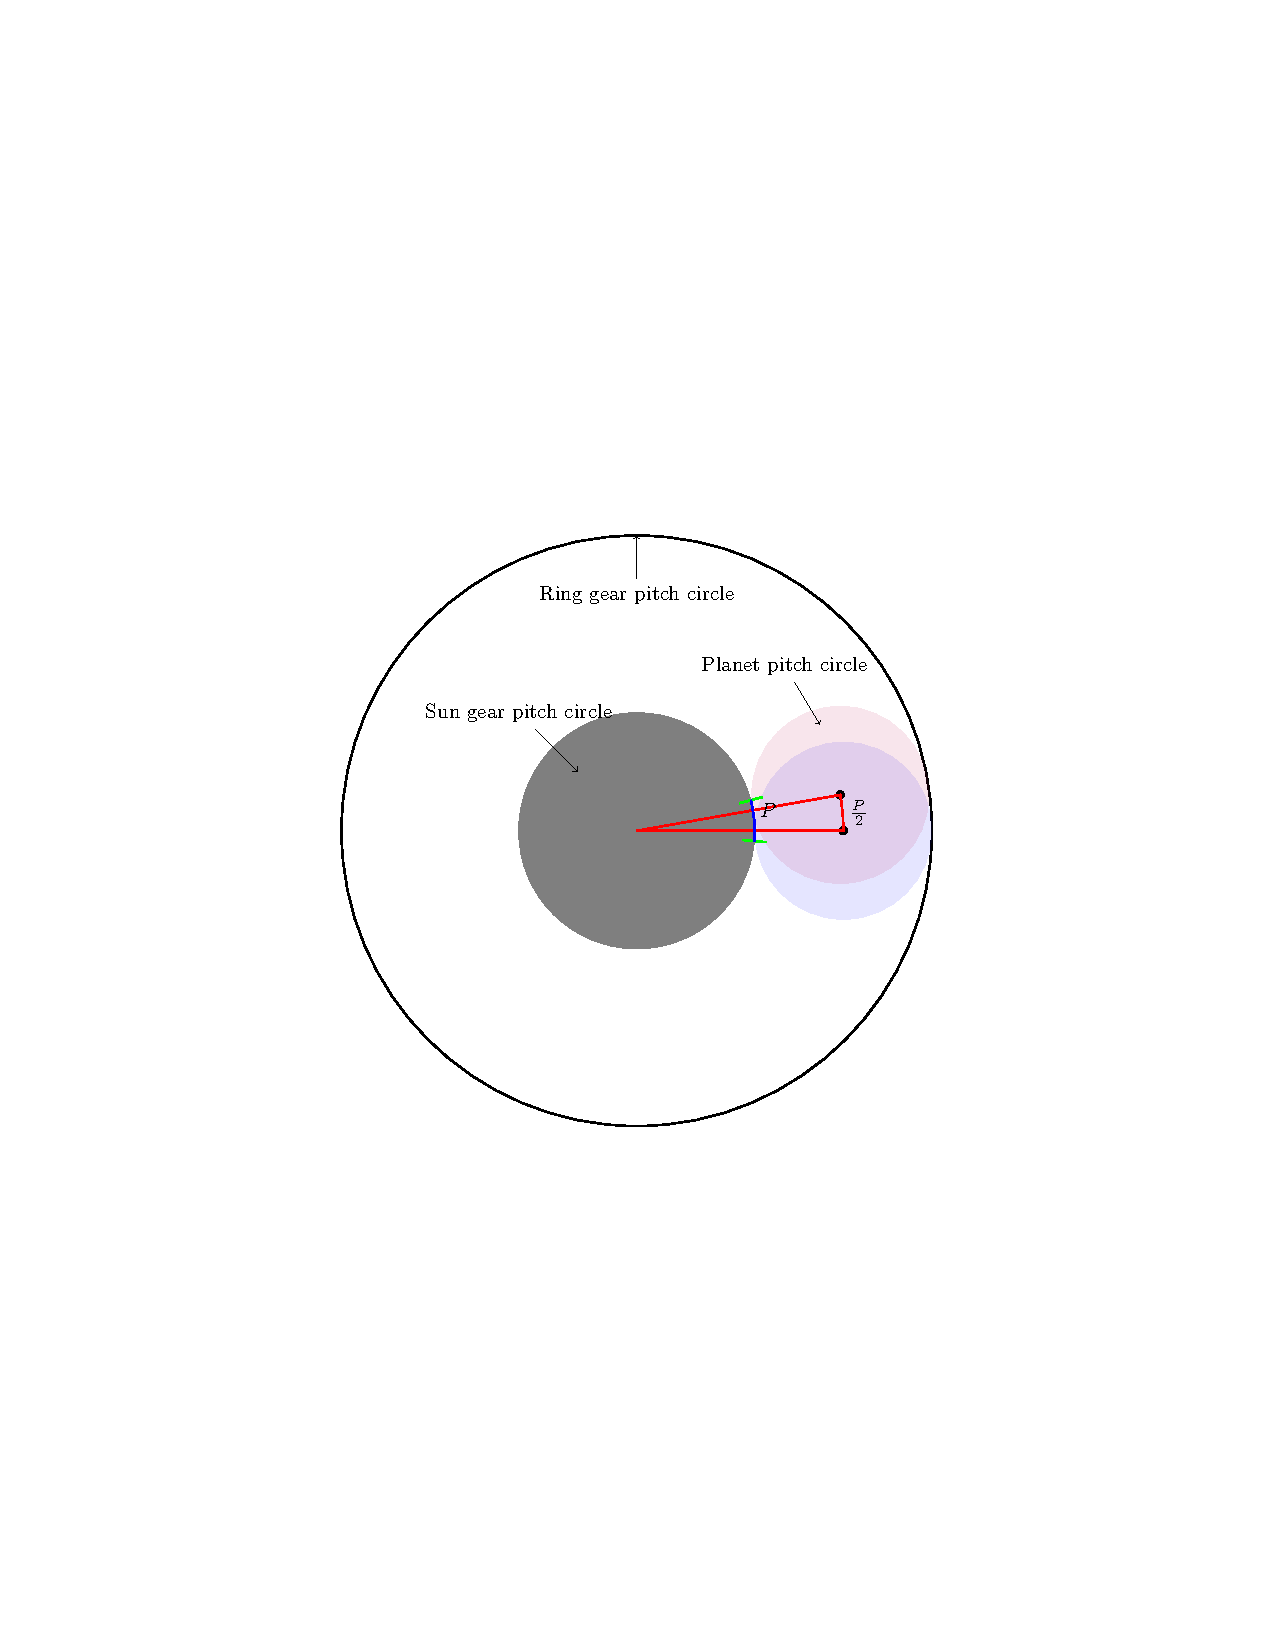
\includegraphics[scale=0.5]{Minimum_angle.pdf}
    \caption{The minimum angle between two adjacent planet possible positions}
    \label{fig_mini_angle}
\end{figure}
\par As shown in Fig. \ref{fig_mini_angle}. The pitch circle of planet gear rolls along the pitch circle of sun gear. When sun gear and ring gear are both fixed, the planet can only assembled at finite discrete angular positions. The minimum angular between two adjacent positions can be calculated as follows. Imagine the sun gear `rotates' an entire tooth, and a planet rotates a distance along with the pinhole circle on the carrier. The transmission ratio between carrier and sun gear is
\begin{equation}
    \operatorname{Transmission\,ratio}=\frac{Z_{\rm s}}{Z_{\rm s}+Z_{\rm r}}
\end{equation}
the angle the sun gear rotates is:$\frac{P}{R_{\rm s}}$, where $P$ is the tooth spacing (base pitch). So the distance the pinhole center rotates is
\begin{equation}
    (R_{\rm s}+R_{\rm p}) \cdot \frac{P}{R_{\rm s}} \cdot \frac{Z_{\rm s}}{Z_{\rm s}+Z_{\rm r}}
    =\frac{R_{\rm s}+R_{\rm p}}{R_{\rm s}+R_{\rm r}} \cdot P
    =\frac{R_{\rm s}+R_{\rm p}}{R_{\rm s}+R_{\rm s}+2R_{\rm p}} \cdot P
    =\frac{P}{2}
\end{equation}
Thus, the angle the planet-carrier rotates is
\begin{equation}
    \lambda=\frac{P}{2} \cdot \frac{1}{R_{\rm p}+R_{\rm s}}
    =\frac{P}{R_{\rm r}+R_{\rm s}}
    \label{equ_carrier_angle}
\end{equation}
According to the definition of module of gear$m=\frac{D}{Z}=\frac{P}{\pi}$, the Eq. (\ref{equ_carrier_angle}) can be rewritten as:
\begin{equation}
    \lambda=\frac{P \cdot 2}{D_{\rm r}+D_{\rm s}}
    =\frac{2 \pi m}{m \cdot ({Z_{\rm r}}+Z_{\rm s})}
    =\frac{2 \pi}{Z_{\rm r}+Z_{\rm s}},
\end{equation}
The planets can only locate finite angular positions with minimum space $\lamda$. When planets locate uniformly at angular positions $\frac{2\pi(i-1)}{M}$, the $Z_{\rm r}+Z_{\rm s}$ must be an integer multiple of planet number $M$.
%% `Elsevier LaTeX' style
\bibliographystyle{elsarticle-num}
\bibliography{My_EndNote_Lib.bib}

\end{document}